%% эта глава концептуально соответсствует предпоследнему слайду моей презентации
%% Universal EDM measurement problems
%% where I have two categories of problems: those solved by using a Spin Wheel,
%% and those having specific solutions
%% the SMP section here covers the SW-solvable problems: stray fields and betatron motion
%% then Spin decoherence and machine imperfections are considered specifically


\chapter{Universal SR EDM measurement problems and their solutions} \label{chpt3:top-level}
 
Universal SR EDM measurement problems can be classified into two groups:
\begin{enumerate*}[(i)]
	\item problems that can ba solved by introducing a spin wheel, and
	\item problems needing specialized solutions.
\end{enumerate*}

Problems of the first category follow from the instability of the invariant spin axis. Among those are,
for example, local electromagnetic field perturbaitons, as well as perturbations to the particle
spin dynamics caused by betatron oscillations. In both cases the particle invariant spin axis deviates from
is equilibrium (closed orbit) orientation for a short period of time.

Problems needing specific solutions include spin decoherence and EDM-faking MDM spin precession. In this part we
analyze the essence of each of these problems, describe their possible solutions, and perform corresponding
simulations.
  
\section{Perturbations to the spin dynamics}\label{chpt3:smp}
\documentclass[a4paper]{jacow}
\usepackage{mathtools}
\usepackage{amsmath}
\usepackage{xfrac}
\usepackage{xparse}
\usepackage{subcaption}
\usepackage{graphicx}
\usepackage{url}
\usepackage{paralist}
\usepackage{multirow}
\usepackage{siunitx}

\let\oldvec\vec
\renewcommand{\vec}{\boldsymbol}
\DeclareDocumentCommand{\bkt}{sm}{\IfBooleanTF{#1}{\left[ #2 \right]}{\left(#2\right)}}
\DeclareDocumentCommand{\ddt}{m}{\frac{\mathrm{d} {#1}}{\mathrm{d} t}}
\DeclareDocumentCommand{\pddx}{mO{t}O{}}{\frac{\partial^{#3} {#1}}{\partial {#2}^{#3}}}
\newcommand{\w}{\omega}
\newcommand{\W}{\Omega}
\newcommand{\avg}[1]{\langle {#1} \rangle}
\newcommand{\nbar}{\bar n}


\begin{document}
\title{Spin Motion Perturbation Effect on the EDM Statistic in the Frequency Domain Method}
\author{A. E. Aksentyev\textsuperscript{1}\thanks{alexaksentyev@gmail.com},
  Institut f\"ur Kernphysik, Forschungszentrum J\"ulich, J\"ulich, Germany \\
  Y. V. Senichev, Institute for Nuclear Research of RAS \\
  \textsuperscript{1}also at National Research Nuclear University ``MEPhI,'' Moscow, Russia}
\maketitle
\footnotetext[2]{a.aksentev@fz-juelich.de}
\begin{abstract}
  The spin precession axis of a particle involved in betatron motion precesses about the invariant spin axis
  defined on the closed orbit (CO). This precession can be observed in polarization data as a rapid,
  small-amplitude oscillation on top of the major effect oscillation caused by the precession of spin
  about the CO axis. The frequency of this latter oscillation is used in the Frequency Domain methodology
  as the EDM observable. It is estimated by fitting polarimetry data by a sine function; the rapid
  oscillations, therefore, constitute a model specification error.
  This model error will introduce a bias into the frequency estimate. In the present work we investigate
  how this bias changes depending on the beam revolution direction, its stability over time, and
  the EDM estimate error introduced by it.
\end{abstract}

\section{Frequency Domain methodology}
Frequency Domain (FD)~\cite{Senichev:FDM} is a Storage Ring method of search for the
Electric Dipole Moment (EDM) of a fundamental particle.~\cite{BNL:SREDM}
It belongs to the Frozen Spin~\cite{BNL:Deuteron2008} category
of such methods, i.e., the Magnetic Dipole Moment (MDM) component of spin precession is minimized. However,
the original Frozen Spin method proposed in~\cite{BNL:Deuteron2008} is a Space Domain
method~\cite[p.~4]{Talman:ElectricRings}: inferences about the EDM are drawn from the change of orientation
of the polarization vector, as measured by the angle between its initial and final orientations. This approach
has the following problems:
\begin{inparaenum}[\itshape a\upshape)]
\item it puts very stringent constraints on the precision of the accelerator optical element alignment, and
\item it poses a challenging task for polarimetry.~\cite[p.~6]{Mane:SpinWheel}
\end{inparaenum}

The former is to minimize the magnitude of
the vertical plane MDM precession frequency:~\cite[p.~11]{BNL:Deuteron2008}
\begin{equation}\label{eq:BNL_syst_err}
\w_{syst} \approx \frac{\mu\avg{E_v}}{\beta c\gamma^2},
\end{equation}
induced by field imperfections. The latter is due to the requirement of detecting a change of about
$5\cdot 10^{-6}$ to the cross section $\varepsilon_{LR}$ in order to get to the EDM sensitivity level
of $10^{-29}~e\cdot cm$.~\cite[p.~18]{BNL:Deuteron2008}

EDM search methods in the Frequency Domain circumvent the above problems: EDM inferences are based
on the rate of change of the aforementioned polarization orientation angle. The polarization vector is made to
roll about a nearly-constant, definite direction vector $\nbar$, with an angular velocity
that is large enough for the beam polarization to be easily measureable at all times. This ``Spin Wheel'' may be
externally applied~\cite{Koop:SW}, or otherwise the machine imperfection fields
may be utilized for the same purpose~\eqref{eq:BNL_syst_err}~\cite{Senichev:FDM}. The latter is made possible
by the fact that $\w_{syst}$ changes sign when the beam revolution direction
is reversed.~\cite[p.~11]{BNL:Deuteron2008}

The frequency of oscillation of the vertical polarization component $P_y$ is estimated
via a fit of the polarimetry data to the model
\begin{equation}\label{eq:fit_model}
  f(t) = a\cdot\sin(\w\cdot t + \delta).
\end{equation}

\section{Problem statement}
\newcommand{\ntrn}{n_{turn}}
Consider the case of a single particle beam. The solution of the T-BMT equation for the
vertical spin-vector component has the general form
\begin{equation}\label{eq:sy_growth_1}
  s_y(t) = \sqrt{\bkt{\frac{\w_y\w_z}{\w^2}}^2 + \bkt{\frac{\w_x}{\w}}^2}\cdot\sin\bkt{\w\cdot t + \delta},
\end{equation}
where $\vec\w = (\w_x, \w_y, \w_z)$ is a function of time as a result of betatron motion.

Using $\vec\w = 2\pi f_{rev}\nu_s\nbar$~\cite[p.~4]{COSY:SpinTuneMapping}, equation~\eqref{eq:sy_growth_1}
can be reformulated in terms of spin tune $\nu_s$ and invariant spin axis $\bar n$:
\begin{equation}\label{eq:main}
  s_y(n_{turn}) = \sqrt{\bkt{\nbar_y\nbar_z}^2 + \nbar_x^2}\cdot\sin\bkt{2\pi\nu_s\cdot\ntrn + \delta},
\end{equation}
where $\nbar = \nbar(\ntrn)$ and $\nu_s = \nu_s(\ntrn)$ are functions of the turn number $\ntrn$.

Sufficiently large variation of~ $\nbar$ and/or $\nu_s$ can lead to model specification systematic error.
Variation in $\nu_s$ is especialy problematic in this regard, as it directly affects the phase of the signal;
however, this problem can be solved by the introduction of sextupole fields into the system,
as described in~\cite{Aksentev:DecohIPAC19}. In this paper we will, therefore, be concerned only with the $\nbar$
variation.

\section{Simulation}
The simulation setup was as follows: a particle, offset from the design orbit in the vertical
direction by 0.3 mm, is injected multiple times into an imperfect
Frozen Spin lattice~\cite{Senichev:Lattices} utilizing sextupoles for
the reduction of spin decoherence caused by vertical plane betatron
oscillations~\cite{Aksentev:DecohIPAC19}. Lattice imperfections are simulated by rotations of the E+B spin
rotator elements. Imperfections introduced this way do not perturb the design orbit.

Each injection, the rotation angles are randomly generated from the
normal distribution $\alpha\sim N(\mu_i, 5\cdot 10^{-6})$ rad, $i\in\{1,\dots,41\}$, where
$\mu_i$ varies in the range $[-1.5\cdot10^{-4}, +2.5\cdot10^{-4}]$. The non-zero expectation values $\mu_i$
simulate the application of a Koop Spin Wheel (SW).~\cite{Koop:SW} The magnitudes of $\mu_i$ and $\sigma_{\alpha}$
are chosen for effect detalization purposes.

Another aspect of the simulation worth noting, is that injection occurs at 270 MeV, while the FS condition
is fullfilled exactly at 270.0092 MeV. Because of that the invariant spin axis $\nbar$
points mainly in the vertical direction (deviating from it by no more than \ang{51} at higher SW roll speeds);
its radial component (the one determining the oscillation amplitude of the vertical spin-vector component)
is relatively small, and all the more susceptible to variation caused by vertical plane betatron motion for that. 

Spin tracking is done in COSY Infinity~\cite{COSYINF:Website}, for $1.2\cdot10^6$ turns; each 800 turns
$\nu_s$ and $\nbar$ are computed (by means of procedure TSS~\cite[p.~41]{COSYINF:BeamPhysMan}) at
the phase space point occupied by the particle at the time, giving us the series $(\nu_s(n), \nbar(n))$.
The corresponding spin vector components $(s_x^{trk}(n), s_y^{trk}(n), s_z^{trk}(n))$,
computed by the tracker (procedure
TR~\cite[p.~41]{COSYINF:BeamPhysMan}), 
constitute the second series used in the analysis.

\section{Analysis}
Using the first series data, we generated the expected $s_y^{gen}(t)$ ``generator'' series according to
equation~\eqref{eq:main}, as well as the ``ideal'' series $s_y^{idl}$, in which
we assumed constant values of $\nu_s = \avg{\nu_s(t)}$ and $\nbar
=\avg{\nbar(t)}$. 

Our hypothesis is that the particle's betatron
motion should introduce a mismatch between the sinusoidal
model~\eqref{eq:fit_model} and tracker data, by varying the direction
of the spin precession axis $\nbar$, and hence the amplitude of the
fitted signal. The ``ideal'' series serves as the baseline of our
analysis, as it's a perfect match to the model; the ``generator''
series incorporates $\nbar$ variation, still remaining within the confines of
the model. The ``tracker'' series is the closest approximation to
real measurement data.

To compare these series with one another, we
\begin{inparaenum}[\itshape a\upshape)]
\item computed and analyzed the residuals
  $\epsilon_1(t) = s_y^{gen}(t) - s_y^{idl}(t)$, and
  $\epsilon_2(t) = s_y^{trk}(t) - s_y^{idl}(t)$;
\item fitted model~\eqref{eq:fit_model} to the three time series and
  compared its goodness-of-fit;
\item computed the standard deviations of $\nbar$ components at each
  spin wheel strength.
\end{inparaenum}

\begin{figure}[h]
  \centering
    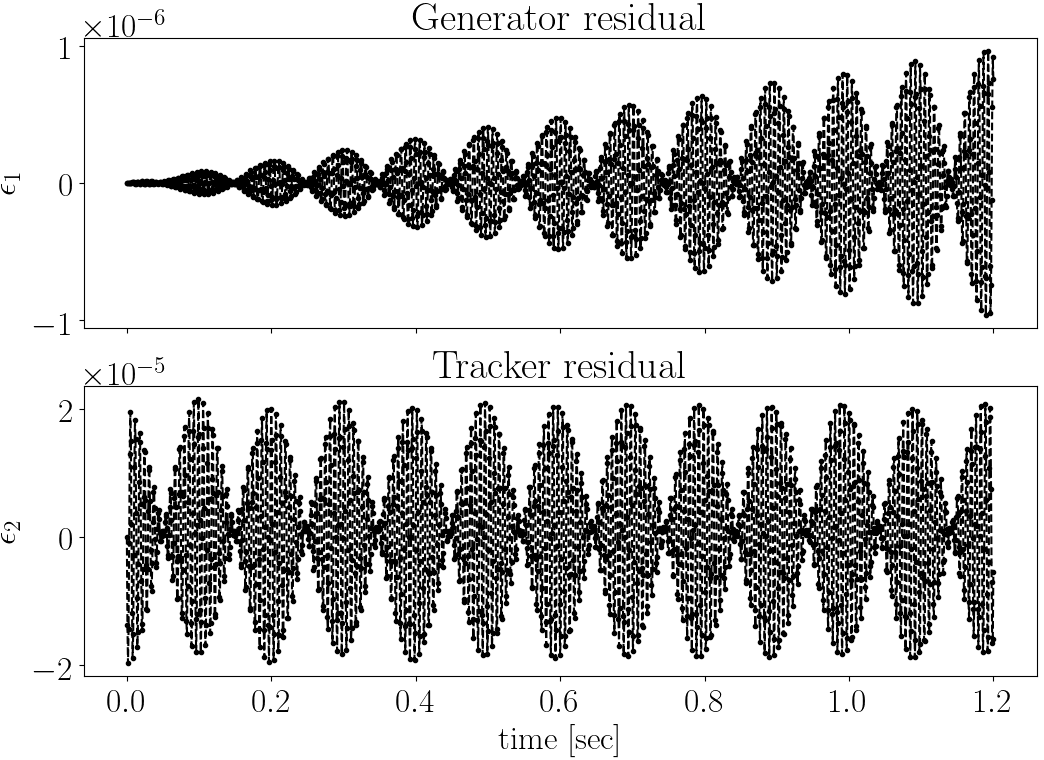
\includegraphics[width=\linewidth]{../img/IPAC19/residual_vs_time(both)}
  \caption{Time series' comparator residual as a function of time.
    Top panel: residual $\epsilon_1$; bottom panel: residual $\epsilon_2$\label{fig:residuals}}
\end{figure}

\begin{figure}[h]
  \centering
  \begin{subfigure}{\linewidth}
    \centering
    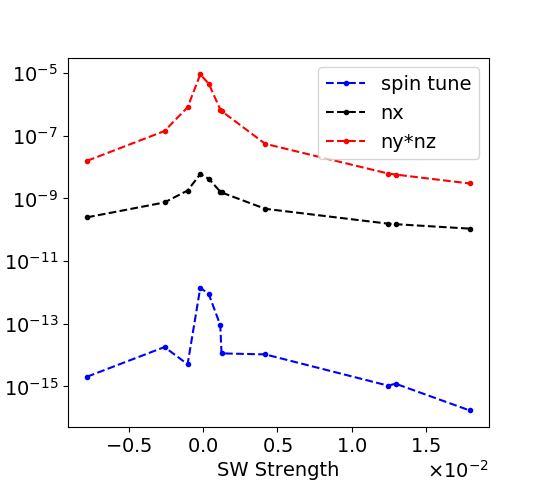
\includegraphics[width=\linewidth]{../img/IPAC19/NBAR_variation_sd_vs_SW}
    \caption{Of the $\nbar$ components\label{fig:sd:nbar}}
  \end{subfigure}
  \begin{subfigure}{\linewidth}
    \centering
    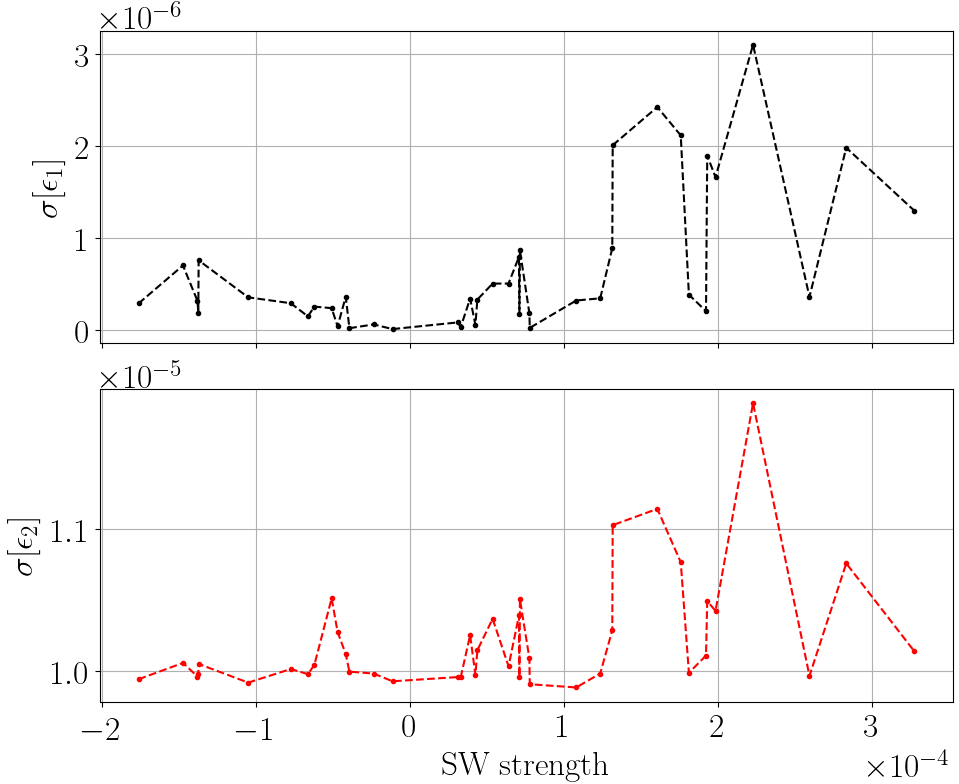
\includegraphics[width=\linewidth]{../img/IPAC19/residual_SD_vs_SW(both)}
    \caption{Of the comparator residuals.
      Top panel: residual $\epsilon_1$; bottom panel: residual $\epsilon_2$\label{fig:sd:res}}
  \end{subfigure}
  \caption{Standard deviations versus relative Spin Wheel strength\label{fig:sd}}
\end{figure}

\begin{table}[h]
  \caption{Model parameter estimates (slowest SW roll)\label{tbl:param_estimates}}
  \begin{tabular}{r|rllr}
    \toprule
    Data & Par. & Value & St.Error & AIC \\
    \midrule
    \multirow{3}{*}{$s_y^{idl}$}
    & $\hat f$ & 4.220359687911 & $6.9\cdot 10^{-11}$ & \multirow{3}{*}{-62093} \\
    & $\hat a$ & 0.12514597851 & $4\cdot 10^{-11}$ & \\
    & $\hat\delta$ & $-1.50\cdot 10^{-8}$ & $4\cdot 10^{-10}$ &\\
    \hline
    \multirow{3}{*}{$s_y^{gen}$}
    & $\hat f$ & 4.2203596911 & $1.9\cdot 10^{-9}$ & \multirow{3}{*}{-52142} \\
    & $\hat a$ & 0.125145979 & $1\cdot 10^{-9}$ & \\
    & $\hat\delta$ & $-1.6\cdot 10^{-8}$ & $1.2\cdot 10^{-8}$ &\\
    \hline
    \multirow{3}{*}{$s_y^{trk}$}
    & $\hat f$ & 4.2203603 & $1.3\cdot 10^{-6}$ & \multirow{3}{*}{-34567} \\
    & $\hat a$ & 0.12514597 & $3.7\cdot 10^{-7}$ & \\
    & $\hat\delta$ & $-4\cdot 10^{-6}$ & $6\cdot 10^{-6}$ &\\
    \bottomrule
  \end{tabular}
\end{table}

What we observe in Figure~\ref{fig:residuals} is that the ``generator'' series is nearly identical
to the ``ideal'' series (even if its frequency is slightly different), with $\epsilon_1 \le 1\cdot10^{-6}$
during run time,
while the ``tracker'' series deviates from it at the level
$\epsilon_2 \le 2\cdot 10^{-5}$. This discrepancy between $\epsilon_1$ and $\epsilon_2$ is observed
systematically across all spin wheel strengths (cf. Figure~\ref{fig:sd:res}), and has no explanation as of yet.

In Figure~\ref{fig:sd:res} we see that the standard deviations of both residuals exhibit the same pattern as
the standard deviation of $\nu_s$ (Figure~\ref{fig:sd:nbar}, bottom panel), but not as that of
the $\nbar$ components. This is an indication that frequency variation is a much more significant factor
in the mismatch between model~\eqref{eq:fit_model} and tracker data, than is the presumed amplitude variation
due to the change of orientation of $\nbar$.

Table~\ref{tbl:param_estimates} characterizes the fit model's goodness-of-fit with respect to the time series,
in the case of the slowest-rolling Koop Wheel.
One observes that the differences between the parameter estimates of all three series are not
statistically significant. Even though variation of the spin precession angular velocity vector worsened
the fit quality of the model, it didn't introduce any statistically-significant bias
into the estimates.

\section{Conclusions}
The question of the influence of betatron motion on the EDM statistic in the FD method should be considered
in view of three circumstances:
\begin{enumerate}
\item The signal amplitude oscillations (as estimated by $\epsilon_2$) are small.
  They occur at the $10^{-4}$ level (when $\sigma_{\alpha}=5\cdot 10^{-4}$), whereas
  the expected polarization measurement error is on the order of percents.
  This means the superposition of this systematic error with the random measurement error
  will exhibit no statistically-significant systematicity.
\item The correllation coefficient between the amplitude and frequency estimates is not significant. The amplitude
  oscillations affect the $\hat a$-estimate foremost; their effect on the $\hat\w$-estimate is secondary, and is
  described by the correlation coefficient. Since it is less than 10\%, even if the oscillations happen to be
  strong enough to affect the amplitude estimate, their effect on the frequency estimate will be reduced by
  at least a factor of 10.
\item This systematic effect is controllable. And this point is the major advantage of the FD methodology.
  By applying an external Spin Wheel, the $\nbar$ oscillations can be continuously minimized
  as much as necessary, without changing the experiment pattern.
\end{enumerate}

\begin{thebibliography}{9}

\bibitem{Senichev:FDM}
  Y. Senichev, A. Aksentev, A. Ivanov, E. Valetov, ``Frequency domain method of the search for
  the deuteron electric dipole moment in a storage ring with imperfections,'' arxiv:1711.06512 [physics.acc-ph]
  \url{https://arxiv.org/abs/1711.06512}.

\bibitem{BNL:SREDM}
  M. Bai et al., SREDM Collaboration website: \url{https://www.bnl.gov/edm/}.

\bibitem{BNL:Deuteron2008}
  D. Anastassopoulos et at., (srEDM Collaboration), ``Search for a permanent electric dipole moment of
  the deuteron nucleus at the $10^{-29}~e\cdot cm$ level,'' proposal as submitted to the BNL PAC, April 2008.

\bibitem{Talman:ElectricRings}
  R. Talman, ``Prospects for Electric Dipole Moment Measurement Using Electrostatic Accelerators,''
  Reviews of Accelerator Science and Technology, A. Chao and W. Chou, editors, Volume 10, 2018, not yet in print.

\bibitem{Mane:SpinWheel}
  S. Mane, ``A distillation of Koop's idea of the Spin Wheel,'' arXiv:1509.01167 [physics]
  \url{http://arxiv.org/abs/1509.01167}.

\bibitem{Koop:SW}
  I. Koop. ``Asymmetric energy colliding ion beams in the EDM storage ring,'' Proc. of IPAC13 (2013).
  \url{http://accelconf.web.cern.ch/accelconf/ipac2013/papers/tupwo040.pdf}.

\bibitem{COSY:SpinTuneMapping}
  A. Saleev et al., (JEDI Collaboration), ``Spin tune mapping as a novel tool to probe
  the spin dynamics in storage rings.'' Phys. Rev. Accel. Beams 20 (2017) no.7, 072801.

\bibitem{Aksentev:DecohIPAC19}
  A. Aksentev, Y. Senichev, ``Spin decoherence in the Frequency Domain Method for the search of a particle EDM,''
  presented at the 10th International Particle Accelerator Conf. (IPAC’19), Melbourne, Australia,
  May. 2019, paper 2738, this conference.

\bibitem{Senichev:Lattices}
  Y. Senichev, S. Andrianov, S. Chekmenev, M. Berz, E.Valetov. ``Investigation of Lattice for Deuteron EDM Ring,''
  Proc. of ICAP15 (2015). \url{http://accelconf.web.cern.ch/AccelConf/ICAP2015/papers/modbc4.pdf}.

\bibitem{COSYINF:Website}
  M. Berz, K. Makino, COSY Infinity website: \url{cosyinfinity.org}.

\bibitem{COSYINF:BeamPhysMan}
  M. Berz, K. Makino. COSY INFINITY 10.0 Beam Physics Manual.

\end{thebibliography} 
\end{document}


\section{Spin decoherence}\label{chpt3:decoherence}
Spin coherence refers to a measure or quality of preservation of polarizaion
in an initially fully-polarized beam.~\cite[p.~205]{Eremey:Thesis}

The spin vectors of a polarized beam injected into a storage ring
begin precessing about the vertical (guiding) field. The precession frequency
depends on the particle equilibrium energy level, which differs across the beam particles.

This circumstance doesn't pose a problem when the beam is vertically polarized;
however, the FS SR EDM measurement method requires that the polarization vector be aligned with
the beam's momentum vector, i.e. lay in the horizontal plane. Hence, spin decoherence is an
inherent problem of the FS methodology.

In the present section we analyze the origins of spin decoherence,
the sextupole method of its suppression, as well as the simulation results
proving the effectiveness of the method.

As an introduction, though, we estimate the spin coherence time required for
the measurement of the EDM in the framework of the space domain methodology.

\documentclass[a4paper]{jacow}

\usepackage{mathtools}
\usepackage{amsmath}
\usepackage{xfrac}
\usepackage{xparse}
\usepackage{subcaption}
\usepackage{graphicx}
\usepackage{url}

\let\oldvec\vec
\renewcommand{\vec}{\boldsymbol}
\DeclareDocumentCommand{\bkt}{sm}{\IfBooleanTF{#1}{\left[ #2 \right]}{\left(#2\right)}}
\DeclareDocumentCommand{\ddt}{m}{\frac{\mathrm{d} {#1}}{\mathrm{d} t}}
\DeclareDocumentCommand{\pddx}{mO{t}O{}}{\frac{\partial^{#3} {#1}}{\partial {#2}^{#3}}}
\newcommand{\w}{\omega}
\newcommand{\W}{\Omega}
\newcommand{\subwidth}{.9\linewidth}
\newcommand{\D}{\Delta}

\begin{document}
\title{Spin decoherence in the Frequency Domain Method for the search of a particle EDM}
\author{A. E. Aksentyev\textsuperscript{1}\thanks{alexaksentyev@gmail.com},
  Institut f\"ur Kernphysik, Forschungszentrum J\"ulich, J\"ulich, Germany \\
  Y. V. Senichev, Institute for Nuclear Research of RAS \\
  \textsuperscript{1}also at National Research Nuclear University ``MEPhI,'' Moscow, Russia}

\maketitle
\begin{abstract}
  Spin coherence refers to a measure of preservation of polarization in an initially polarized beam. The spin vector of a particle injected into a storage ring starts to precess about the vertical magnetic field vector in accordance with the Thomas-BMT equation. The precession frequency is dependent on the equilibrium-level energy, which differs across the beam particles. This does not pose a problem when the initial polarization is vertical; however, the Frozen Spin Storage Ring EDM search method requires beam polarization along the momentum vector, i.e., in the horizontal plane. 
  
  In the present work we analyze the source of decoherence, and investigate the way it can be suppressed in the horizontal plane in a perfectly aligned ring by means of sextupole fields. We also consider the case of an imperfect ring, the vertical plane decoherence introduced by field imperfections, and its effect on the EDM estimator used in the Frequency Domain method.
\end{abstract}

\section{Spin dynamics in a storage ring}
The dynamics of a spin-vector $\vec s$ in a magnetic field $\vec B$ and an electrostatic field $\vec E$ is described by the Thomas-BMT equation. Its generalized version, accounting for the effect of the particle's electric dipole moment, can be written in the rest frame as:
\begin{subequations}
  \begin{align}
    \ddt{\vec s} &= \vec s\times \bkt{\vec\W_{MDM} +\vec\W_{EDM}}, \label{eq:TBMT_main}
    \intertext{where the magnetic (MDM) and electric (EDM) dipole moment angular velocities $\vec\W_{MDM}$ and $\vec\W_{EDM}$ }
    \vec\W_{MDM} &= \frac qm \bkt*{G\vec B - \bkt{G - \frac{1}{\gamma^2-1}}\frac{\vec E\times\vec\beta}{c}},\label{eq:TBMT_MDM} \\
    \vec\W_{EDM} &= \frac qm \frac\eta2 \bkt*{\frac{\vec E}c + \vec\beta\times \vec B}.\label{eq:TBMT_EDM}
  \end{align}
\end{subequations}
In the above equations, $m,~q,~G=(g-2)/2$ are, respectively, the mass, charge, and magnetic anomaly of the particle; $\beta = \dfrac{v_0}{c}$ is its normalized speed; $\gamma$ its Lorentz-factor. The EDM factor $\eta$ is defined by the equation $d = \eta\frac{q}{2mc}$, in which $d$ is the particle EDM, $s$ its spin.

In the standard formalizm one operates with the spin transfer matrix~\cite[p.~4]{COSY:SpinTuneMapping}
\[
\boldsymbol{t}_R = \exp\bkt{-i\pi\nu_s\vec\sigma\cdot\bar n} = \cos\pi\nu_s - i (\vec\sigma\cdot\bar n)\sin\pi\nu_s,
\]
where $\nu_s = \sfrac{\W_s}{\W_{cyc}}$, the ratio of the particle's spin precession frequency to its cyclotron frequency, is termed \emph{spin tune}, and $\bar n$, termed the \emph{invariant spin axis}, defines the spin precession axis. They relate to the spin precession angular velocity as in $\vec\W_s = \w_{cyc}\cdot \nu_s\bar n$.

\section{Origin of decoherence}
Spin decoherence in a particle beam is a result of the difference of the particles' spin precession angular velocities ($\vec\W_s$), which, in turn, is caused by the difference of their orbit lengths.

The longitudinal dynamics of a particle on the reference orbit in a storage ring is described by the system of equations:
\begin{equation}
  \begin{cases}
    \ddt{\D\varphi} &= -\w_{RF}\eta\delta, \\
    \ddt{\delta} &= \frac{q V_{RF}\w_{RF}}{2\pi h\beta^2E}\bkt{\sin\varphi - \sin\varphi_0}.
  \end{cases}
\end{equation}
In the equations above, $\D\varphi = \varphi-\varphi_0$ and  $\delta = (p-p_0)/p_0$ are the deviations
of the particle's phase and normalized momentum from those of the reference particle;
$V_{RF}$, $\w_{RF}$ are the amplitude and frequency of the RF field;
$\eta = \alpha_0 - \gamma^{-2}$ is the slip-factor, where $\alpha_0$ is
the momentum compaction factor defined by $\sfrac{\Delta L}{L} = \alpha_0\delta$, $L$ being the orbit length;
$h$ is the harmonic number; $E$ the total energy of the particle.

The solutions of this system form a family of ellipses in the $(\varphi, \delta)$-plane, all centered at the point
$(\varphi_0,\delta_0)$. However, if one considers a particle involved in betatron oscillations, and uses a higher-order Taylor expansion of the momentum compaction factor $\alpha = \alpha_0 + \alpha_1\delta$, the first equation of the system transforms into:~\cite[p.~2579]{Senichev:IPAC13}
\[
\ddt{\varphi} = -\w_{RF} \bkt*{\bkt{\frac{\Delta L}{L}}_\beta + \bkt{\alpha_0 + \gamma^{-2}}\delta + \bkt{\alpha_1 - \alpha_0\gamma^{-2} + \gamma^{-4}}\delta^2},
\]
where $\bkt{\frac{\Delta L}{L}}_\beta = \frac{\pi}{2L}\bkt*{\varepsilon_xQ_x + \varepsilon_yQ_y}$, is the betatron motion-related orbit lengthening; $\varepsilon_x$ and $\varepsilon_y$ are the horizontal and vertical beam emittances, and $Q_x$, $Q_y$ are the horizontal and vertical tunes.

The solutions of the transformed system are no longer centered at the same single point. Orbit lengthening and momentum deviation cause an equilibrium-level momentum shift~\cite[p.~2581]{Senichev:IPAC13}
\begin{equation}\label{eq:EquLevMom_shift}
\Delta\delta_{eq} = \frac{\gamma_0^2}{\gamma_0^2\alpha_0 - 1}\bkt*{\frac{\delta_m^2}{2}\bkt{\alpha_1 - \alpha_0\gamma^{-2} + \gamma_0^{-4}} + \bkt{\frac{\Delta L}{L}}_\beta},
\end{equation}
where $\delta_m$ is the amplitude of synchrotron oscillations.

The equilibrium energy level, associated with the momentum shift~\eqref{eq:EquLevMom_shift}, termed the \emph{effective Lorentz-factor}, is\cite{Senichev:FDM}
\begin{equation}\label{eq:EffectiveGamma}
\gamma_{eff} = \gamma_0 + \beta_0^2\gamma_0\cdot\Delta\delta_{eq},
\end{equation}
where $\gamma_0$, $\beta_0$ are the Lorentz-factor and normalized speed of the reference particle.

From the T-BMT equation~\eqref{eq:TBMT_MDM}, and the equation of cyclotron frequency in a magnetic field $\w_{cyc} = \frac qm \frac B\gamma$, spin tune $\nu_s = \gamma_{eff}G$; therefore, the variation of orbit lengths over the beam particles casues a spin tune dispersion, and consequently --- spin decoherence.

\section{Sextupole field suppression of decoherence}
A sextupole field with gradient $ S_{sext} = \frac{1}{B\rho} \pddx{B_y}[x][2]$, has a two-fold effect on decoherence:
\begin{itemize}
\item it directly affects the particles' orbit lengths: $\bkt{\frac{\Delta L}{L}}_{sext} = \mp \frac{S_{sext}D_0\beta_{x,y}\varepsilon_{x,y}}{L}$, and
\item it modifies the lattice's momentum compaction factor: $\Delta \alpha_{1,sext} = -\frac{S_{sext}D_0^3}{L}$.
\end{itemize}
Above, $\beta_{x,y}$ are the horizontal, vertical beta-functions; $D(s) = D_0(s) + D_1(s)\delta$ is the dispersion function; $B\rho$ is magnetic rigidigy.

Consequently, in order to reduce decoherence associated with horizontal, and vertical betatron oscillations, and with synchrotron oscillations, correcting sextupoles must be placed, respectively, in the maxima of the $\beta_x$-, $\beta_y$- and $D$-functions.
\section{Simulation of decoherence suppression}
In the following simulation we used a Frozen Spin-type lattice represented in Figure~\ref{fig:FSBNL_lattice}. All optical elements are perfectly aligned, i.e., there's no spin precession about the radial coordinate system axis. Particles were injected at 270 MeV kinetic energy, which is the frozen spin energy for the deuteron in this lattice. Computations were performed using the COSY Infinity code.~\cite{COSY:Website} Spin tune and invariant spin axis Taylor expansions were computed up to 5th order. Simulation results are presented in Figure~\ref{fig:decoherence_suppression_sim}.

\begin{figure}[h!]
  \centering
  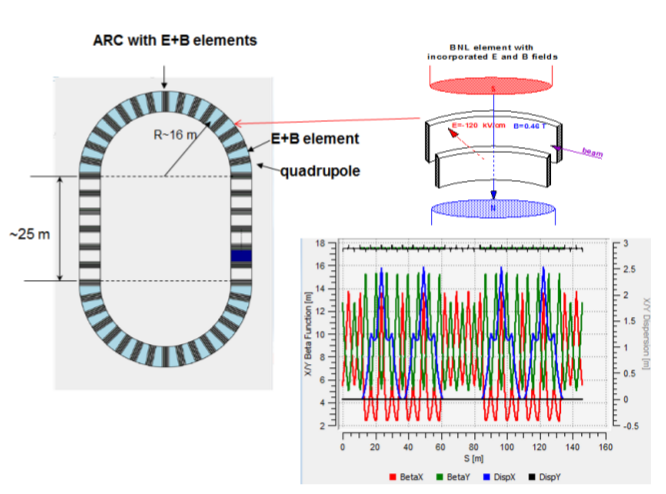
\includegraphics[width=\linewidth]{../img/Lattice/BNL}
  \caption{Frozen spin-type lattice used in simulations.\label{fig:FSBNL_lattice}}
\end{figure}
\begin{figure}[ht]
  \centering
  \begin{subfigure}{\subwidth}
    \centering
    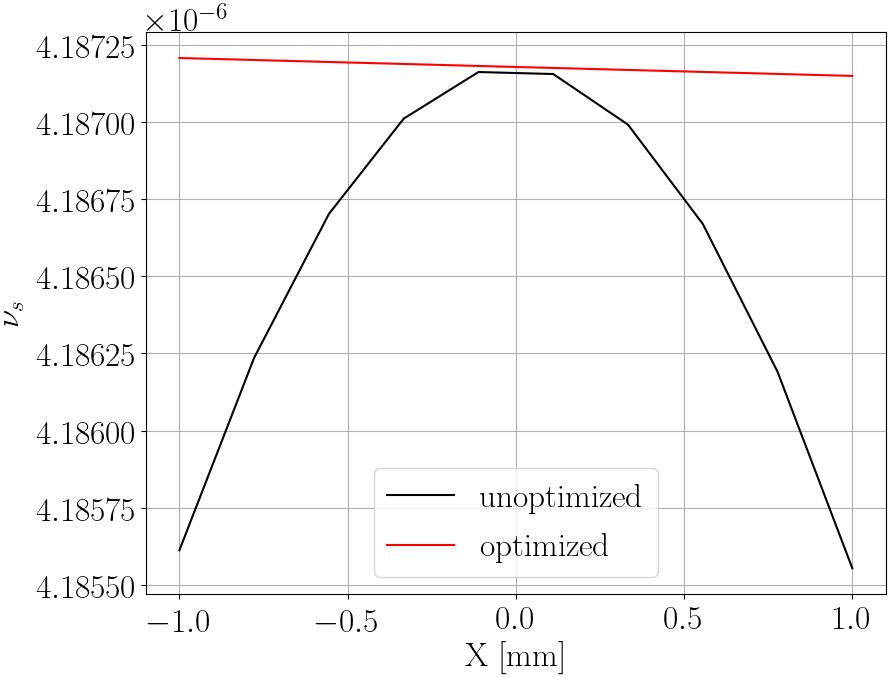
\includegraphics[width=\linewidth]{../img/IPAC19/spin_tune_decoh_x_offset}
    \caption{For particles involved in horizontal betatron oscillation only\label{fig:st_decoh_horizontal}}
  \end{subfigure}
  \begin{subfigure}{\subwidth}
    \centering
    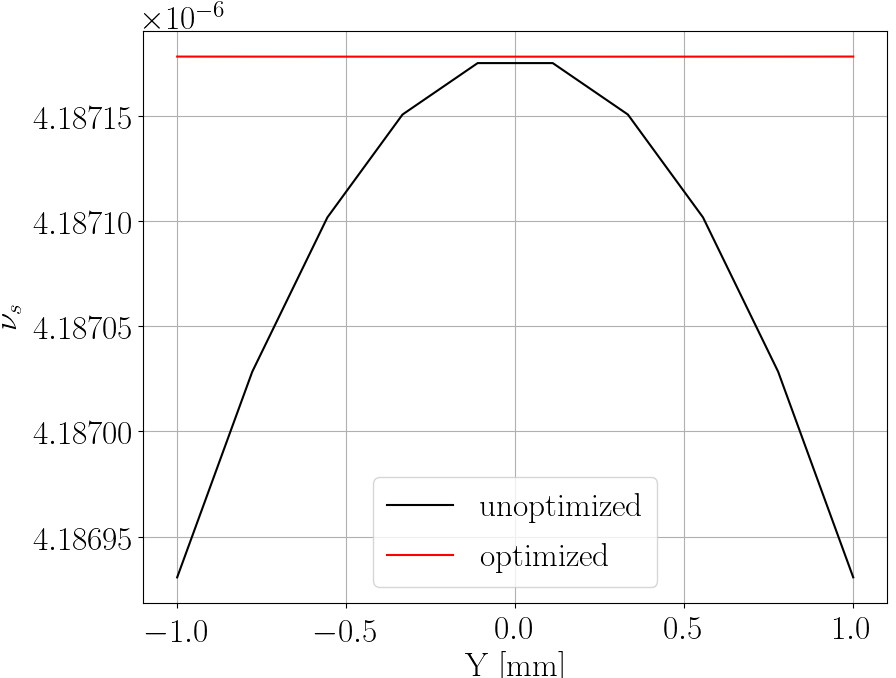
\includegraphics[width=\linewidth]{../img/IPAC19/spin_tune_decoh_y_offset}
    \caption{For particles involved in vertical betatron oscillation only}
  \end{subfigure}
  \begin{subfigure}{\subwidth}
    \centering
    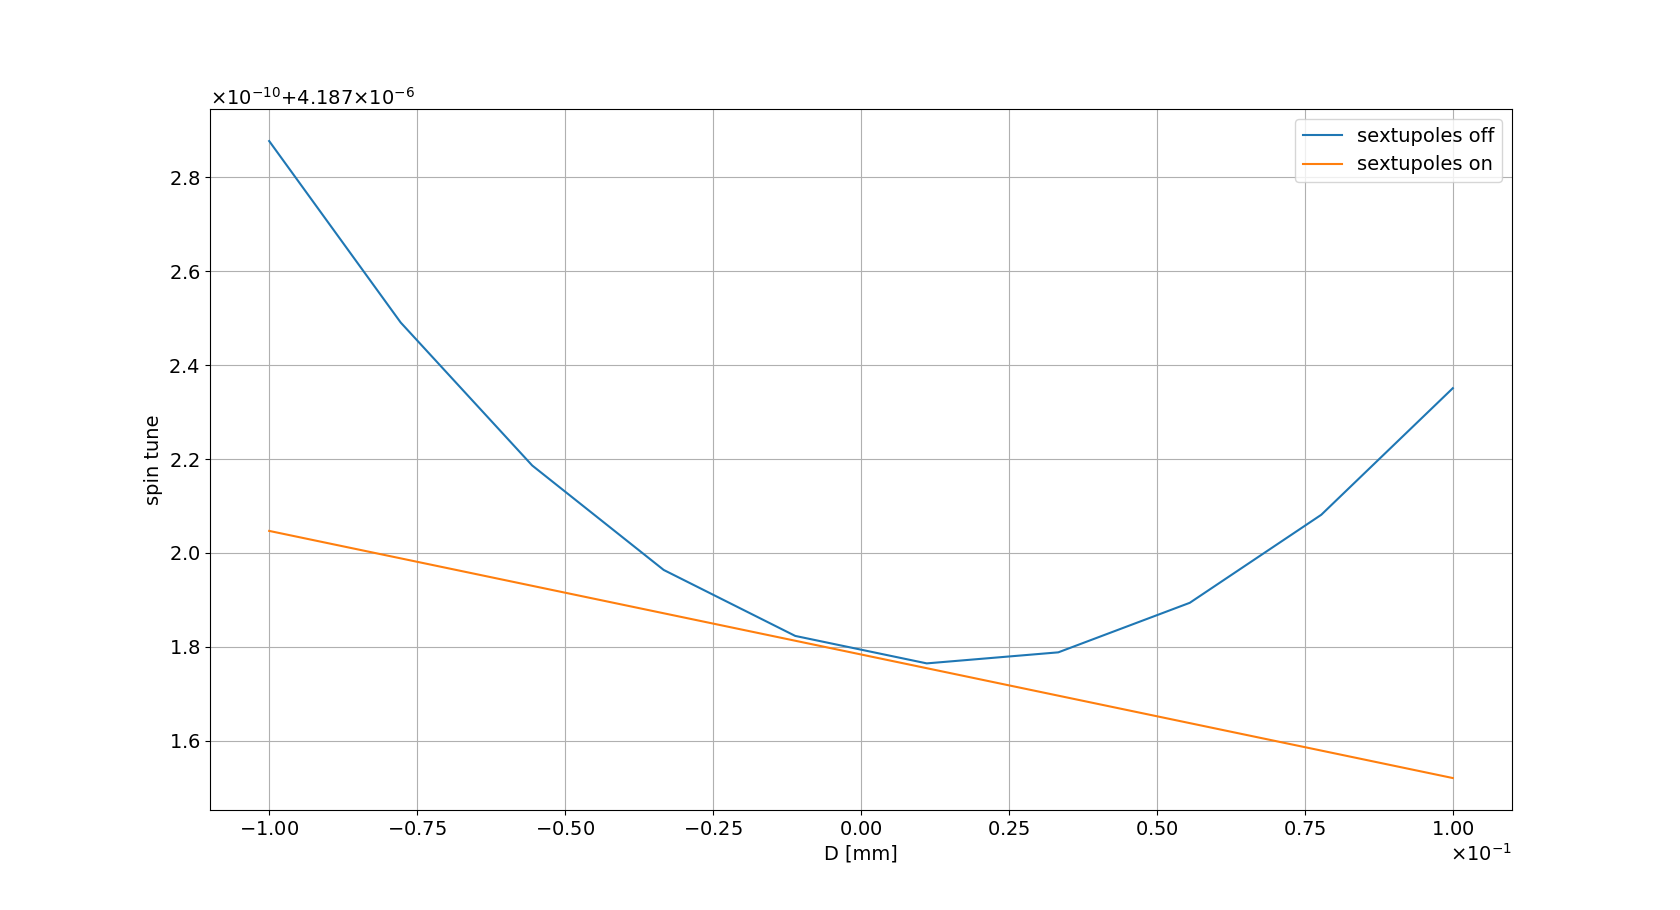
\includegraphics[width=\linewidth]{../img/IPAC19/spin_tune_decoh_d_offset}
    \caption{For particles involved in synchrotron oscillation only\label{fig:st_decoh_synchrotron}}
  \end{subfigure}
  \caption{Spin tune a as function of initial horizontal, vertical, or momentum offset of the particle, with and without correcting sextupoles\label{fig:decoherence_suppression_sim}}
\end{figure}

\section{Simulation of decohrence in an imperfect lattice}
In this simulation we rotated the E+B elements about the optic axis by angles generated from the normal distribution $\alpha \sim N(0, 5\cdot 10^{-4})$ rad. The value $\sigma_\alpha = 5\cdot 10^{-4}$ is a realistic~\cite{Senichev:FDM} element alignment error standard deviation. A rotation of an E+B element does not cause a perturbation of the closed orbit, since the net Lorentz force is kept constant.

\begin{figure}[ht]
  \centering
  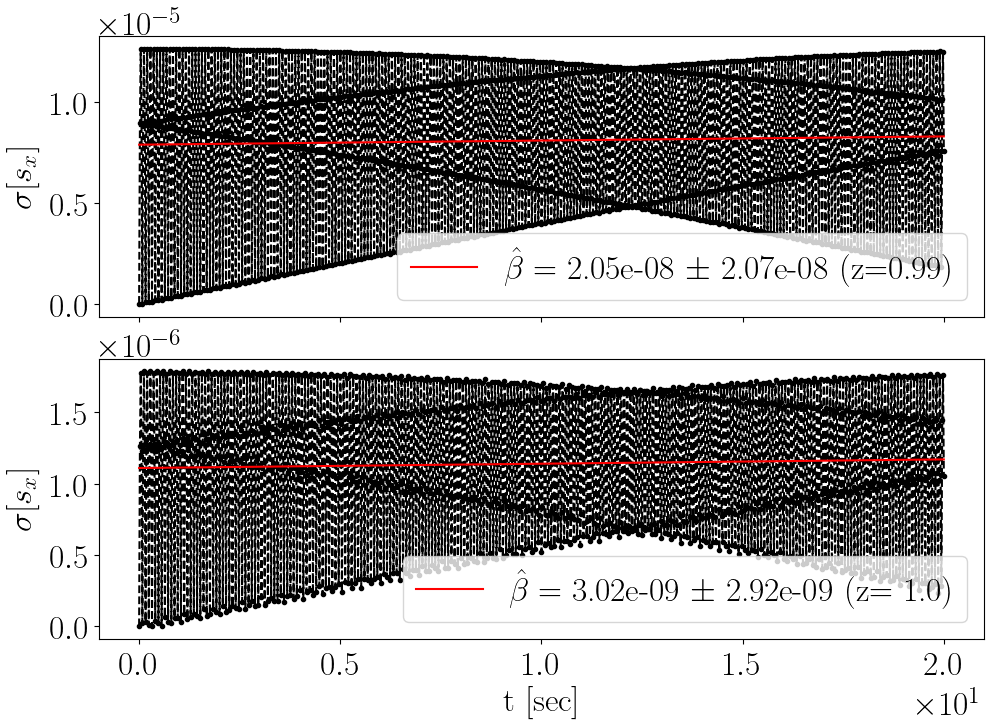
\includegraphics[width=\linewidth]{../img/IPAC19/SX_decoh_20sec_both}
  \caption{Standard deviation of the radial spin vector components in a particle bunch.
    Top panel: sextupoles are turned off; bottom panel: sextupoles are turned on\label{fig:decoh_rms_sx}}
\end{figure}

Figure~\ref{fig:decoh_rms_sx} shows the standard deviation of the radial spin-vector components in a particle bunch before and after turning on correcting sextupoles. Because an imperfect lattice was used, the particles' spin-vectors precess in the vertical plane at a rapid pace, and hence the RMS-value of $S_x$ is an oscillating function that does not show a long-term growth trend (slope estimate $(2 \pm 2)\cdot 10^{-8}$ 1/sec); there's no decoherence in the horizontal plane. Use of correcting sextupoles further reduces the amplitude of the $\sigma_{S_x}$-oscillations.

\begin{figure}[ht]
  \centering
  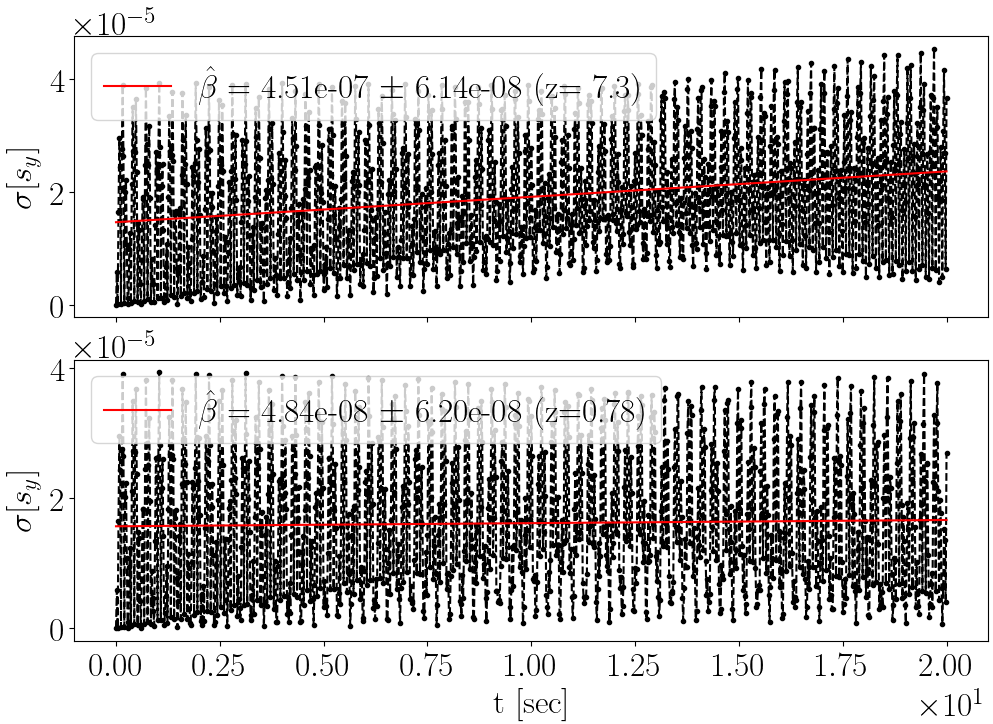
\includegraphics[width=\linewidth]{../img/IPAC19/SY_decoh_20sec_both}
  \caption{Standard deviation of the vertical spin vector components in a particle bunch.
    Top panel: sextupoles are turned off; bottom panel: sextupoles are turned on\label{fig:decoh_rms_sy}}
\end{figure}

Figure~\ref{fig:decoh_rms_sy} shows the same statistic for the vertical components. One observes a presence of a long-term trend (slope estimate $(4.5 \pm 0.6)\cdot 10^{-7}$ 1/sec) prior to turning on correcting sextupoles (Figure~\ref{fig:decoh_rms_sy}, top panel). Sextupole correction does not reduce the amplitude of the $\sigma_{S_y}$-oscillations, but it does remove the long-term trend (Figure~\ref{fig:decoh_rms_sy}, bottom panel,
slope estimate $(5 \pm 6) \cdot 10^{-8}$ 1/sec).

\section{Conclusions}
Spin decoherence is a major problem for any experiment aiming to measure the EDM of an elementary particle using the storage ring method,~\cite{BNL:Deuteron2008} as it drastically reduces the possible measurement cycle time. In the present work we have described the mechanism by which it arises, and a method by which it can be suppressed. We have shown that by means of this method the parabolic dependence of spin tune on the particle coordinate can be removed. The remaining linear decoherence effect observed in Figures~\ref{fig:st_decoh_horizontal} and~\ref{fig:st_decoh_synchrotron} is suppressed by use of an RF-cavity.

\begin{thebibliography}{9}
  
\bibitem{COSY:SpinTuneMapping}
  A. Saleev et al., (JEDI Collaboration), ``Spin tune mapping as a novel tool to probe the spin dynamics in storage rings.'' Phys.Rev.Accel.Beams 20 (2017) no.7, 072801

\bibitem{Senichev:IPAC13}
  Y. Senichev, R. Maier, D. Zyuzin, N. Kulabukhova, (JEDI Collaboration), ``Spin tune decoherence effects in electro- and magnetostatic structures.'' Proc. of IPAC13 (2013).

\bibitem{Senichev:FDM}
  Y. Senichev, A. Aksentev, A. Ivanov, E. Valetov, ``Frequency domain method of the search for the deuteron electric dipole moment in a storage ring with imperfections.'' In review.

\bibitem{COSY:Website}
  M. Berz, Kyoko Makino, COSY Infinity. \url{cosyinfinity.org}

\bibitem{BNL:Deuteron2008}
  D. Anastassopoulos et at., (srEDM Collaboration), ``Search for a permanent electric dipole moment of the deuteron nucleus at the $10^{-29}~e\cdot cm$ level,'' proposal as submitted to the BNL PAC, April 2008.
  
\end{thebibliography}
\end{document}


\section{Machine imperfections error}\label{chpt3:imperfections}
Systematic errors due to physical imperfections of the accelerator lattice, including
optical element misalignments, are causative to an EDM-faking signal 
related to MDM spin precession~\cite[p.~230]{Eremey:Thesis} Rotational magnet misalignments 
are particularly problematic in this respect, since they induce parasitic horizontal magnetic field
components $B_x$ and $B_z$, both of which precess spin in the vertical plane; the one in which
the EDM is searched for.

Y. Senichev made analytical estimates~\cite{Senichev:FDM}  of the radial component of
the spin precession angular velocity. From the T-BMT equation, and the expression for
the Lorentz force, its radial component can be expressed as 
\begin{equation}
\SD{\W_x^{MDM}} = \frac{q}{m\gamma}\frac{G+1}{\gamma}\frac{\SD{B_x}}{\sqrt{n}},
\end{equation}
where $n$ is the number of tilted spin-rotator elements,~\footnote{The estimates were made for
the FS lattice described in section~\ref{chpt2:lattice:FS_BNL}.} and $\SD{B_x} = B_y \SD{\delta h}/L$, 
with the misalignment error standard deviation $\SD{\delta h}$. Assuing $\SD{\delta h} = 100$~$\mu$m, 
and spin-rotator length $L=1$ ~m, $\SD{\W_x^{MDM}} \approx 100$ rad/sec.~\cite{Senichev:FDM}

We analyzed the particle spin dynamics in the imperfect FS and QFS lattices using COSY Infinity.~\cite{COSYINF:Website} 
Our simulation results tend to confirm the above estimates.


\paragraph{Imperfection field implementation}\label{chpt3:imperfections:implementation}
When implementing machine imperfections we followed recommendations given in~\cite[p.~235]{Eremey:Thesis}. 
A small perturbation of the magnetic field acts like a proportional rotation of the spin vector.
For this reason we implemented the E+B element tilt as a product between the element's spin transfer matrix
and the corresponding rotation matrix, a ``spin kick.'' Such an implementation guarantees the preservation of 
the closed orbit. This orbit preservation is physically grounded in the fact that when a spin-rotator
is tilted, there emerges a compensating electric field keeping the Lorentz force constant.

According to equation~\eqref{eq:TBMT_MDM}, a change in the MDM precession angular velocity
associated with the presence of a parasitic magnetic field $(B_x, 0, B_z)$ is
\begin{align*}
	\Delta\W_{MDM} &= \frac qm G \cdot (B_x, 0, B_z),
	\intertext{hence the spin kick angle}
	\Theta_{kick} &= t_0\Delta\W_{MDM},
\end{align*}
where $t_0 = L/v_0$ is the reference particle's time of flight through the element.

\subsection{Tilt distribution dependence} \label{chpt3:imperfections:magnitude}
This series of simulations was carried out in order to prove (or reject) the validity of two theses
concerning the machine imperfection systematic error:
\begin{enumerate*}[(1)]
	\item the induced MDM spin precession angular velocity component is independent of the particular
	element tilt distribution, and depends only on the mean tilt angle; and
	\item this dependence is linear.
\end{enumerate*}

The simulation was set up as follows: in the FS lattice described in section~\ref{chpt2:lattice:FS_BNL} 
 E+B elements were randomly tilted about the optic axis by angles $\Theta_{tilt}$.
 After building the third-order spin and orbital transfer maps, we computed the Taylor expansions of the
 spin tune and spin precession axis (SPA). The zero-order terms of the Taylor expansions represent the spin tune and SPA
 of the reference particle.
 
 The reference particle spin precession angular velocity is calculated 
 according to equation:~\cite[p.~4]{COSY:SpinTuneMapping}
\[
\vec\W = 2\pi/\tau_0\cdot \nu_s \cdot \bar n,
\]
where $\tau_0 = f^{-1}_{rev} = 10^{-6}$ seconds is the particle's time of flight through the full lattice.

The simulation was carried out 11 times; each time the spin-rotator tilt angles were picked
from a normal distribution $N(\mu_0\cdot(i-5), \sigma_0)$, where 
$\mu_0 = 10\cdot \sigma_0 = 10^{-4}$ rad, $i\in\lbrace0,\dots, 10\rbrace$. The simulation
results are plotted in Figure~\ref{fig:Linearity_test_shifting_gauss}.

\begin{figure}[!h]
	\centering
	\begin{subfigure}{\linewidth}
		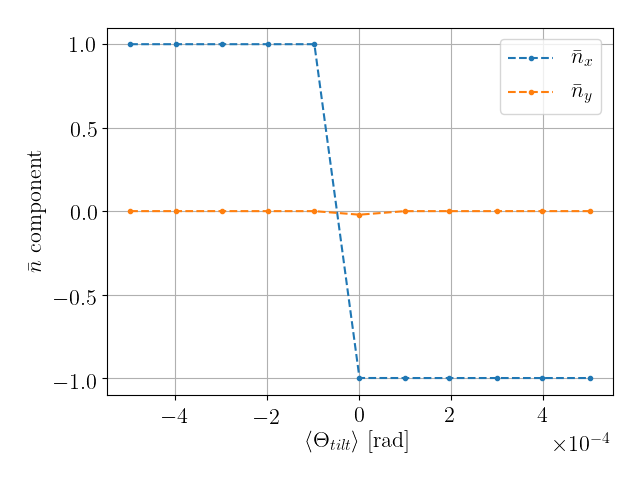
\includegraphics[height=.35\paperheight]{images/fake_signal_sim/linearity_test_shifting_gauss_nbar}
		\caption{Spin precession axis $\nbar$ components.}
	\end{subfigure}
	\begin{subfigure}{\linewidth}
		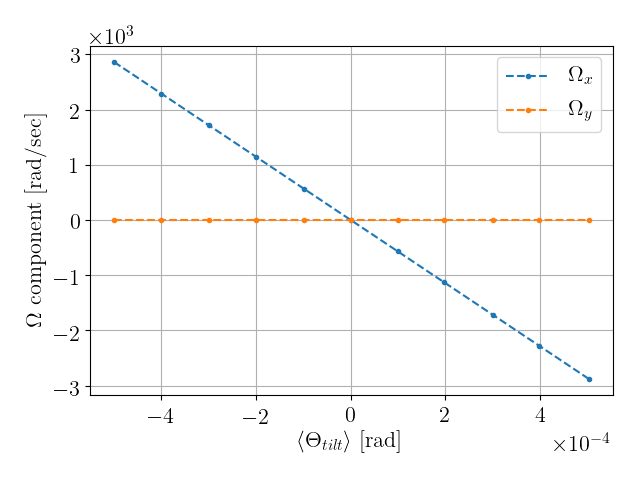
\includegraphics[height=.35\paperheight]{images/fake_signal_sim/linearity_test_shifting_gauss_freq}
		\caption{Angular velocity $\vec\W$ components.}
	\end{subfigure}
	\caption{Reference particle's spin precession axis and angular velocity components as
		 functions of the mean E+B element tilt angle. Element tilts are normally distributed.
		Color identifies the component; radial (blue) and vertical (orange).\label{fig:Linearity_test_shifting_gauss}}
\end{figure}

One can observe from the figure that a tilt distribution at which the mean tilt angle is equal to $10^{-4}$ radians, the
beam polarization vector precesses in the vertical plane at the rate of 500 rad/sec. This agrees with the estimates
mentioned above (section~\ref{chpt3:imperfections}), because in them a tilt error standard deviation of $10^{-4}$ rad 
is assumed at 100 tilted elements. In that case, the mean tilt angle standard deviation is $10^{-5}$, and hence MDM
precession occurs at a rate up to 50 rad/sec with a probability 67\%, and up to 100 rad/sec with a probability 95\%.

Figure~\ref{fig:Linearity_test_compensated} shows the results of a simulation in which six randomly-picked
E+B elements were pair-wise tilted by opposite angles, while one element was tilted by an angle
$\mu_i = (i-5)\cdot 10^{-6}$ rad, $i\in\lbrace0,\dots,10\rbrace$. 

Both simulations were done at the strict FS energy 270.0092 MeV.\footnote{At this energy, in the ideal lattice, 
	$\nu_s$ and $\nbar$	are undefined in the beam rest frame used in COSY Infinity.
	This corresponds to the situation when spin does not precess in any plane (either horizontal or vertical), 
	which corresponds to the realization of the 3D FS condition in an ideal lattice.} One can see that the compensated
elements do not contribute to the spin precession.

\begin{figure}[!h]
	\centering
	\begin{subfigure}{\linewidth}
		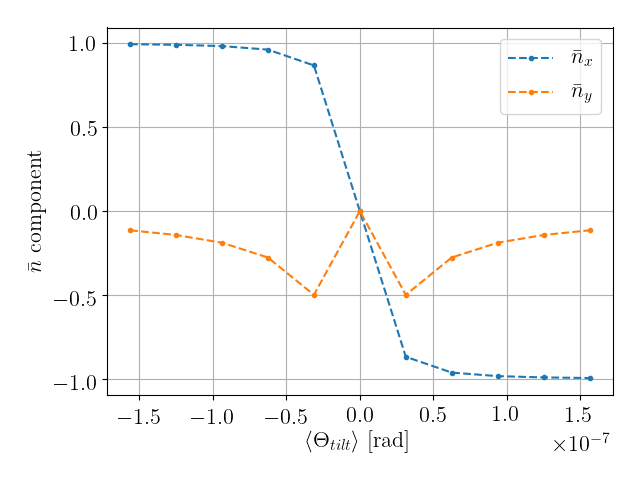
\includegraphics[height=.35\paperheight]{images/fake_signal_sim/linearity_test_compensated+microrad_nbar}
		\caption{Spin precession axis $\nbar$ components.}
	\end{subfigure}
	\begin{subfigure}{\linewidth}
		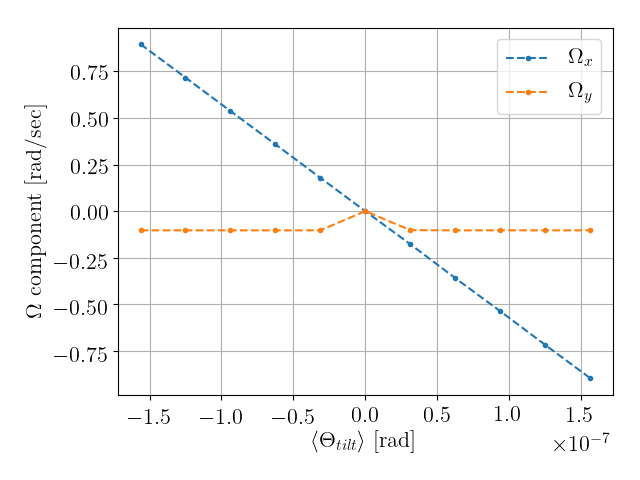
\includegraphics[height=.35\paperheight]{images/fake_signal_sim/linearity_test_compensated+microrad_freq}
		\caption{Angular velocity vector $\vec\W$ components.}
	\end{subfigure}
	\caption{Reference particle's spin precession axis and angular velocity components as
		functions of the mean E+B element tilt angle. Three mutually-compensated tilt pairs plus an uncompensated
		rotation.
		Color identifies the component; radial (blue) and vertical (orange)\label{fig:Linearity_test_compensated}}
\end{figure}

\subsection{Comparison of the CW vs CCW beams' spin precession angular velocities}\label{chpt3:imperfections:CW_vs_CCW}
In Figure~\ref{fig:Lin_test_rel_diff} we plotted the relative difference between the CW and CCW beams' radial SPA/angular velocity
components in the case of both the normally-distributed and mutually-compensated tilt cases.

For the raidal SPA component the relative difference was computed as
\[
\delta\bar n_x = \frac{\bar n_x^{CW}(\avg{\Theta_{tilt}}) - \bar n_x^{CCW}(\avg{\Theta_{tilt}})}{\bar n_x^{CW}(\avg{\Theta_{tilt}})};
\]
for the angular velocity:
\[
\delta\W_x = \frac{\W_x^{CW}(\avg{\Theta_{tilt}}) - \W_x^{CCW}(\avg{\Theta_{tilt}})}{\W_x^{CW}(\avg{\Theta_{tilt}})}.
\]

In the figures, one can observe that in either case both beams' SPA is oriented the same way; 
there is some difference between the beams' spin tunes, but it stays below the percent level. 
The spin tune difference grows bigger as the
spin wheel roll rate (proportional to the mean tilt angle) gets slower. 
The spin tune difference may indicate that
the lattice is asymmetric, with respect to the spin dynamics, relative to the beam circulation direction (i.e. time reversal).
It may be explained by a difference between the CW and CCW beams' closed orbits.

\begin{figure}[!h]
	\centering
	\begin{subfigure}{\linewidth}
		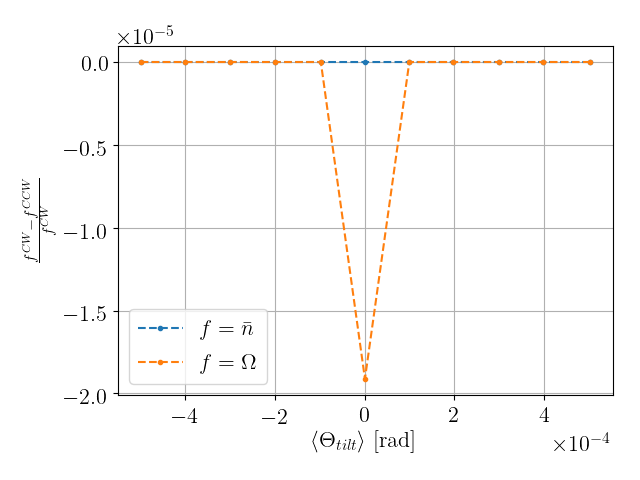
\includegraphics[height=.35\paperheight]{images/fake_signal_sim/linearity_test_shifting_gauss_rel_diff}	
		\caption{Normally distributed E+B element tilts.}
	\end{subfigure}
	\begin{subfigure}{\linewidth}
		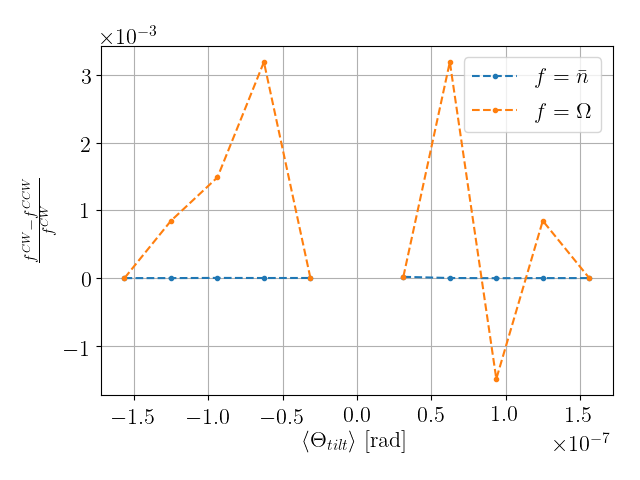
\includegraphics[height=.35\paperheight]{images/fake_signal_sim/linearity_test_compensated+microrad_rel_diff}
		\caption{Mutually-compensated element tilts.}
	\end{subfigure}
	\caption{Relative difference between the CW and CCW beams' spin precession axis and angular velocity radial components.
		Color marks the compared variable: spin precession axis (blue) and abgular velocity (orange).\label{fig:Lin_test_rel_diff}}
\end{figure}


\section{Guide field flipping}\label{chpt3:GFF}

Two aspects of the problem need to be paid attention to:
\begin{enumerate}
\item What needs to be kept constant from one measurement cycle to the next;
\item How it can be observed.
\end{enumerate}

The goal of flipping the direction of the guide field is to accurately reproduce the radial component
of the MDM spin precession frequency induced by machine imperfection fields. This point should not be overlooked:
a mere reproduction of the \emph{magnetic field strength} would not suffice, since the injection point of
the beam's centroid,
and hence its orbit length --- and, via equations~\eqref{eq:EffectiveGamma} and~\eqref{eq:spin_tune_vs_gamma},
spin tune, --- is subject to variation. (Apart from that, the accelerating structure might not be symmetrical,
in terms of spin dynamics, with regard to reversal of the beam circulation direction.)

What needs to be reproduced, therefore, is not the field strength, but the effective Lorentz factor of
the centroid.

Regarding the second question, we mentioned earlier that the Koop Wheel roll rate
is controlled through measurement of the horizontal plane spin precession frequency. 
This plane was chosen because the EDM angular velocity vector points
(mainly) in the radial direction; its vertical component is due to machine imperfection fields,
and is small compared to
the measured EDM effect. Therefore, in first approximation, when we manipulate the vertical component of the 
combined spin precession angular velocity, we manipulate the vertical component of the MDM
angular velocity vector.

The effective Lorentz factor calibraion procedure consists in the following.

\documentclass[a4paper]{jacow}

\usepackage{mathtools}
\usepackage{amsmath}
\usepackage{xfrac}
\usepackage{xparse}
\usepackage{subcaption}
\usepackage{graphicx}
\usepackage{url}
\usepackage{paralist}

\let\oldvec\vec
\renewcommand{\vec}{\boldsymbol}
\DeclareDocumentCommand{\bkt}{sm}{\IfBooleanTF{#1}{\left[ #2 \right]}{\left(#2\right)}}
\DeclareDocumentCommand{\ddt}{m}{\frac{\mathrm{d} {#1}}{\mathrm{d} t}}
\DeclareDocumentCommand{\pddx}{mO{t}O{}}{\frac{\partial^{#3} {#1}}{\partial {#2}^{#3}}}
\newcommand{\w}{\omega}
\newcommand{\W}{\Omega}
\newcommand{\avg}[1]{\langle {#1} \rangle}

\begin{document}
\title{Simulation of the Guide Field Flipping Procedure for the Frequency Domain Method}
\author{A. E. Aksentyev$^1$\footnotemark[2], Institut f\"ur Kernphysik, Forschungszentrum J\"ulich, J\"ulich, Germany \\$^1$ also at National Research Nuclear University ``MEPhI,'' Moscow, Russia}
%\author{$^1$ also at National Research Nuclear University ``MEPhI,'' Moscow, Russia}
%\ead{a.aksentev@fz-juelich.de}
\maketitle
\footnotetext[2]{a.aksentev@fz-juelich.de}
\begin{abstract}
  The spin vector of a particle injected into a perfectly aligned storage ring precesses about the vertically-orientated guide field. In the presence of an Electric Dipole Moment (EDM), the spin precession axis acquires a proportional radial component.
  However, in an imperfect ring, rotational magnet misalignments induce a radial component to the spin precession axis, related to the Magnetic Dipole Moment (MDM). In the Frequency Domain Method, this additional precession is dealt with by consecutively injecting the beam in opposite directions, and constructing the EDM estimator as the sum of the clockwise and counter-clockwise vertical plane precession frequencies. Since the radial MDM component changes sign when the magnetic field direction is reversed, it cancels in the sum, leaving only the EDM effect. 
  In order to reproduce the guide field magnitude with a precision sufficient for the cancellation of the MDM effect, we propose to calibrate the guide field via the horizontal plane precession frequency. In the present work we describe the algorithm of the field flipping procedure, and make a numerical simulation.
\end{abstract}

\section{Spin dynamics in a storage ring}
The dynamics of a spin-vector $\vec s$ in a magnetic field $\vec B$ and an electrostatic field $\vec E$ is described by the Thomas-BMT equation. Its generalized version, accounting for the effect of the particle's electric dipole moment, can be written in the rest frame as:
\begin{subequations}
  \begin{align}
    \ddt{\vec s} &= \vec s\times \bkt{\vec\W_{MDM} +\vec\W_{EDM}}, \label{eq:TBMT_main}
    \intertext{where the magnetic (MDM) and electric (EDM) dipole moment angular velocities $\vec\W_{MDM}$ and $\vec\W_{EDM}$ }
    \vec\W_{MDM} &= \frac qm \bkt*{G\vec B - \bkt{G - \frac{1}{\gamma^2-1}}\frac{\vec E\times\vec\beta}{c}},\label{eq:TBMT_MDM} \\
    \vec\W_{EDM} &= \frac qm \frac\eta2 \bkt*{\frac{\vec E}c + \vec\beta\times \vec B}.\label{eq:TBMT_EDM}
  \end{align}
\end{subequations}
In the above equations, $m,~q,~G=(g-2)/2$ are, respectively, the mass, charge, and magnetic anomaly of the particle; $\beta = \sfrac{v_0}{c}$ is its normalized speed; $\gamma$ its Lorentz-factor. The EDM factor $\eta$ is defined by the equation $d = \eta\frac{q}{2mc}$, in which $d$ is the particle EDM, $s$ its spin.

%% In the standard formalizm one operates with the spin transfer matrix~\cite[p.~4]{COSY:SpinTuneMapping}
%% \[
%% \boldsymbol{t}_R = \exp\bkt{-i\pi\nu_s\vec\sigma\cdot\bar n} = \cos\pi\nu_s - i (\vec\sigma\cdot\bar n)\sin\pi\nu_s,
%% \]
%% where $\nu_s = \sfrac{\W_s}{\W_{cyc}}$, the ratio of the particle's spin precession frequency to its cyclotron frequency, is termed \emph{spin tune}, and $\bar n$, termed the \emph{invariant spin axis}, defines the spin precession axis. They relate to the spin precession angular velocity as in $\vec\W_s = \w_{cyc}\cdot \nu_s\bar n$.

\section{BNL Frozen Spin method}
The original method for the measurement of the electric dipole moment of an elementary particle was first proposed by the Storage Ring EDM Collaboration~\cite{BNL:SREDM} of the Brookhaven National Laboratory. In the proposed method,~\cite{BNL:Deuteron2008} a longitudinally-polarized beam is injected into a storage ring designed on the basis of the Frozen Spin (FS) concept: by applying a radial electric field $E_r = \frac{GB_yc\beta\gamma^2}{1-G\beta^2\gamma^2}$,~\cite[p.~10]{BNL:Deuteron2008} the MDM component in~\eqref{eq:TBMT_main} is set to zero: $\vec\W_{MDM} = \vec 0$. Then, any tilting of the beam polarization vector out of the horizontal plane is attributed to the presence of an EDM; specifically, the vertical component $P_y$ grows as
\[
P_y =  P\frac{\W_{edm}}{\W}\sin\bkt{\W t + \Theta_0} \approx P\W_{EDM}\cdot t,
\]
where $\W = \sqrt{\W_{EDM}^2 + \W_{MDM}^2}$.~\cite[p.~8]{BNL:Deuteron2008}

This method has two inherent weaknesses, due to the smallness of the hypothesized EDM value:
\begin{inparaenum}[\itshape a\upshape)]
\item the expected polarization tilt angle after 1,000 seconds is on the order of microradians,~\cite[p.~18]{BNL:Deuteron2008} which is a difficult task for polarimetry~\cite[p.~6]{Mane:SpinWheel} and
\item the main systematic effect, $\W_{syst} \approx \frac{\mu\avg{E_y}}{c\beta\gamma^2}$ ($\mu$ being the MDM of the particle)~\cite[p.~10]{BNL:Deuteron2008} must be reduced to less than $\W_{EDM}$ if one is to measure the polarization tilt angle.
\end{inparaenum}
The considered systematic error is caused by accelerator element misalignment error. For a practical value of 100$\mu$m of element installation error, this means a $\W_{syst}$ on the order of 50 rad/sec.~\cite{Senichev:FDM}

Both these problems can be mitigated if the net precession \emph{frequency}, instead of \emph{phase}, is used as the EDM observable.

\section{Frequency Domain Method}
The Frequency Domain Methodology (FDM)~\cite{Senichev:FDM} was designed specifically to address the problem with element misalignment error. The FS condition condition is fulfilled as in the BNL method; however, instead of the polarization tilt angle, the combined MDM+EDM precession frequency is measured in two cases: once when the beam is injected clockwise, and once counter-clockwise. The EDM-effect is extracted by comparing the measured frequencies. When the guide field polarity is reversed $\vec B \mapsto -\vec B$, $\vec\beta \mapsto -\vec\beta$, and $\vec E \mapsto \vec E$, the precession frequency components change thus:
\begin{subequations}
  \begin{align}
    \W_x^{CW/CCW} &= \W_x^{MDM, CW/CCW} + \W_x^{EDM, CW/CCW}, \\
    \W_x^{MDM, CW} &= -\W_x^{MDM, CCW} \equiv \W_x^{MDM}, \label{eq:FDM_CW_CCW_MDM} \\
    \W_x^{EDM, CW} &= \W_x^{EDM, CCW} \equiv \W_x^{EDM},
    \intertext{and the EDM estimator}
    \hat\W_x^{EDM} &:= \frac12\bkt{\W_x^{CW} + \W_x^{CCW}} \label{eq:FDM_estimator} \\
    &= \W_x^{EDM} + \underbrace{\frac12\bkt{\W_x^{MDM, CW} + \W_x^{MDM, CCW}}}_{\varepsilon \to 0}.
  \end{align}
\end{subequations}

In order to guarantee that $\varepsilon$ is less than the required EDM measurement precision, i.e. that the equation~\eqref{eq:FDM_CW_CCW_MDM} holds with sufficient accuracy, a guide field flipping algorithm has been devised, that uses the horizontal plane precession frequency as a means to calibrating the guide field. 

\section{Calibration algorithm}
The main concern in flipping the direction of the guide field is to accurately reproduce the radial component of teh MDM spin precession frequency due to element misalignment.

The spin precession frequency components are defined by the following equation:~\cite[p.~4]{COSY:SpinTuneMapping}
\[
(\W_x, \W_y, \W_z) = 2\pi\cdot f_{rev} \cdot \nu_s \cdot \bar n,
\]
where $f_{rev}$ is the particle cyclotron frequency, $\nu_s$ and $\bar n$ are its spin tune and invariant spin axis respectively.

We consider the case of a lattice utilizing sextupole elements in order to reduce spin tune dispersion.~\cite{Aksentev:DecohIPAC19} In such a lattice, both $\nu_s$ and $\bar n$ are uniform over a large area of the transverse cross-section of the vacuum tube (and also momentum deviation), and therefore we will assume that all the beam particles share the spin tune and precession axis defined on the reference (closed) orbit.

The reference orbit $\nu_s^{CO}$ is determined by the orbit length, and $\bar n^{CO}$ is determined by both the orbit length and electromagnetic field orientation. When flipping the guide field, the field orientation is preserved, and so the problem of reproducing the MDM angular velocity component comes down to reproducing $\nu_s^{CO}$. This is done directly via reproducing $\W_y^{MDM}$:
in the initial state, $\W_x\gg \W_y, \W_z$ and $\bar n^{CO}\approx \hat x$. Using a spin-rotator (Wien filter), we 
suppress precession about $\hat x$; simultaneously we offset the beam energy from the ``frozen'' value (this is done so as to avoid the unstable ``3D Frozen Spin'' state).  When changing the beam energy, we also adjust the guide field strength accordingly, so as to preserve the reference orbit. Horizontal precession becomes dominant, and $\bar n^{CO}\approx \hat y$. After reversing the guide field polarity, we adjust its strength once again to fulfill the FS condition. Then, after turning off the spin-rotator, and brining the beam energy back to its original level, we get $\bar n^{CO}\approx -\hat x$, $\nu_s^{CCW} = \nu_s^{CW}$, i.e., MDM precession occurs at the same rate as before, but in the opposite direction.

One known systematic error in this procedure is the vertical component $\W_y^{EDM} \propto \vec\beta\times\vec B_x$, where $B_x$ is the misalignment error field, but this error is by default less than the estimated radial EDM frequency component, and can be neglected.

\section{Simulation}

\section{Conclusions}


\begin{thebibliography}{9}

\bibitem{BNL:SREDM}
  M Bai et al., SREDM Collaboration website: \url{https://www.bnl.gov/edm/}

\bibitem{BNL:Deuteron2008}
  D. Anastassopoulos et at., (srEDM Collaboration), ``Search for a permanent electric dipole moment of the deuteron nucleus at the $10^{-29}~e\cdot cm$ level,'' proposal as submitted to the BNL PAC, April 2008.

\bibitem{Mane:SpinWheel}
  S Mane, ``A distillation of Koop's idea of the Spin Wheel.'' arXiv:1509.01167 [physics] \url{http://arxiv.org/abs/1509.01167}
  
\bibitem{Senichev:FDM}
  Y. Senichev, A. Aksentev, A. Ivanov, E. Valetov, ``Frequency domain method of the search for the deuteron electric dipole moment in a storage ring with imperfections.'' In review.

\bibitem{COSY:SpinTuneMapping}
  A. Saleev et al., (JEDI Collaboration), ``Spin tune mapping as a novel tool to probe the spin dynamics in storage rings.'' Phys.Rev.Accel.Beams 20 (2017) no.7, 072801

\bibitem{Aksentev:DecohIPAC19}
  A Aksentev, Y Senichev, ``Spin decoherence in the Frequency Domain Method for the search of a particle EDM.'' Proc. of IPAC19 (2019).
  
%% \bibitem{Senichev:IPAC13}
%%   Y. Senichev, R. Maier, D. Zyuzin, N. Kulabukhova, (JEDI Collaboration), ``Spin tune decoherence effects in electro- and magnetostatic structures.'' Proc. of IPAC13 (2013).

%% \bibitem{COSY:Website}
%%   M. Berz, Kyoko Makino, COSY Infinity website: \url{cosyinfinity.org}


  
\end{thebibliography}
\end{document}


\section{Spin tune equivalence of trajectories of equal effective Lorentz factor}\label{sec:spin_tune_traj_equivalence}
In the context of the spin wheel roll direction change procedure, it is important to consider the question
of the CW and CCW beams' equivalence in trems of their spin dynamics.

Our analysis starts from Statement 1: particles having an equal effective Lorentz factor value have equal
spin tunes, i.e. are equivalent in their spin dynamics. This is a consequence of
equation~\eqref{eq:spin_tune_vs_gamma}.

In the next sections we will consider two formulations of Statement 1:
\begin{enumerate}[A.]
	\item when interpreting the effective L-factor as the expectation value of the particle energy;
	\item the multivariate function $\nu_s(x, a, y, b, \ell, \delta)$ is agnostic to the paricle's
          trajectory in the transverse phase planes $(x,a)$, and $(y,b)$, that is, it can be reduced
          to a multivariable function $\nu_s(\g*)$.
\end{enumerate}

\subsection{Formulation A}

In this section we will consider Statement 1, interpreting the effective Lorentz factor as the expectation value
of a particle's Lorentz factor.

In order to test this formulation we carried our the following simulation: we injected three 10-particle
bunches (X, Y, and D) into the ideal FS lattice. The orbital and spin transfer maps were computed
up to the third-order Taylor expansion; the particle injection energy was 270~MeV. The X-bunch particles
were uniformly distributed along the radial axis in the range $\pm 1$ mm; those of the Y-bunch, along the vertical
axis in the range $\pm 1.318$ mm;~\footnote{This range was chosen in order to equalize the transverse
emittances of the particles. The initial coordinate offset determines the betatron oscillation amplitude $A$,
which is related to the beta function $\beta$ and transverse emittance $\epsilon$ as in
$A = \sqrt{\epsilon \beta}$.} the D-bunch particles were distributed by $\Delta K/K_0$ in the range $\pm 10^{-4}$.
Then, spin tracking was done for 12,000 turns, with data recorded every 80 turns.

The recorded data were: 
\begin{enumerate}[(i)]
	\item the particle phase space coordinate $\vec z~=~(x,x',y,y',\ell, \delta)$, where
$\ell~=~-(t-t_0)v_0\frac{\gamma_0}{1+\gamma_0}$ is its longitudinal phase offset, 
$\delta~=~\Delta K/K$ is the energy offset;
\item spin tune $\nu_s(\vec z)$.
\end{enumerate}
Based on these data we computed the particles' time-average spin tune $\avg{\nu_s}$,
energy offset  $\avg{\Delta K/K}$, and longitudinal and transverse emittances.

Simulation results are presented in Figure~\ref{fig:stune_traj_equ_main}. The top panel is a plot of $\avg{\nu_s}$ as a function of $\avg{\Delta K/K}$ for the betatron-oscillating bunches when the sextupoles
are turned off. One can see from the figure that, at the same mean energy level, the horizontal plane
 betatron oscillating particles have a different spin tune from that of the vertical plane betatron
oscillating particles. This means, as far as we can tell, that Statement 1 in formulation A is disproved.

We hypothesized that the difference in the plotted lines' slopes is related to the
\emph{spatial dependence} of the momentum compaction factor.

This hypothesis is based on our analysis of the sextupole field suppression effects' signatures, described
in detail in section~\ref{sec:sext_decoh_suppression_effect_analysis}. In order to test this hypothesis we
repeated the experiment at different values of the GSX sextupole gradient, taken from
the range $\pm 5\cdot 10^{-3}$. The simulation results are shown in Figure~\ref{fig:stune_traj_equ_main}.
The same dependence is plotted as previously, but only for the X-bunch.
As one can see, when the gradient is varied the slope varies with it. The same behavior as was
observed in section~\ref{sec:sext_decoh_suppression_effect_analysis}.

\begin{figure}[h]
	\centering
	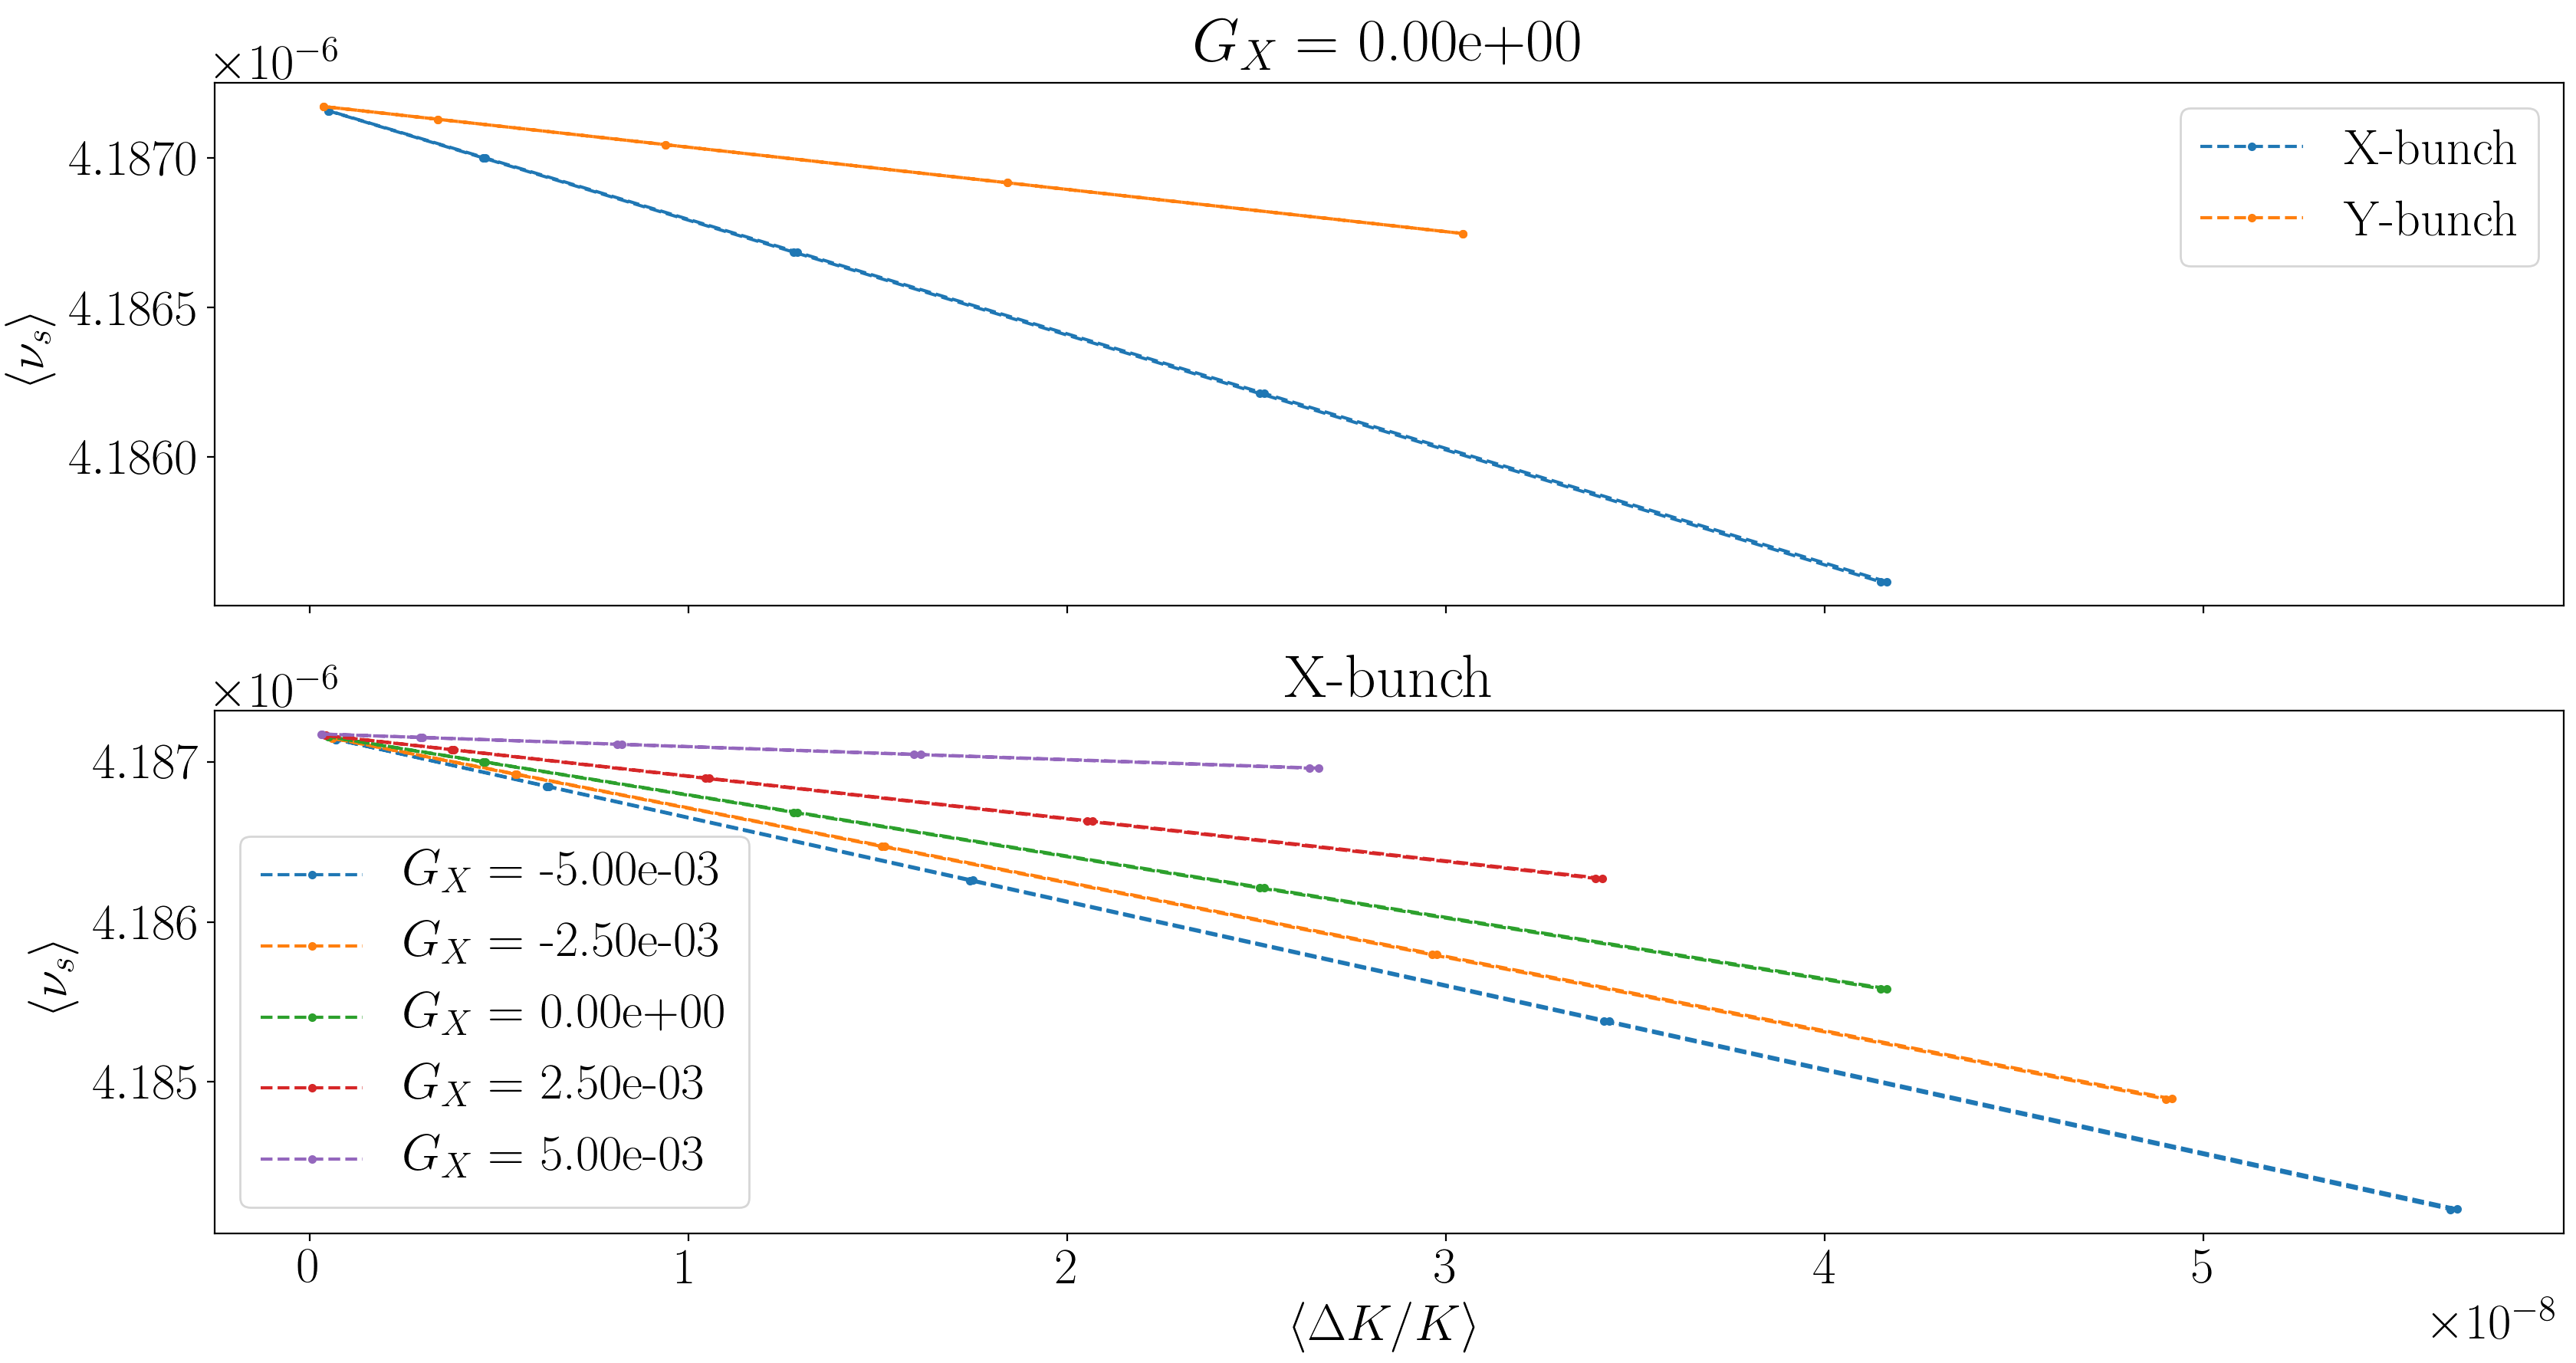
\includegraphics[height=.3\paperheight]{images/stune_traj_equ/part1/stune_vs_equ_energy}
	\caption[Mean spin tune level veresus mean kinetic energy level.]{Particle mean spin tune level
        as a function of its mean kinetic energy level. Top panel: sextupoles are off for both injected bunches.
        Bottom panel: X-bunch dependencies at different GSX gradients.\label{fig:stune_traj_equ_main}}
\end{figure}

In order to check the hypothesis about the spatial dependence of the momentum compaction factor we computed
the dependencies of the mean energy levels of the X- and Y-bunch particles on their betatron tune-normalized
transverse emittances (Fiugre~\ref{fig:equ_nrg_vs_emittance}).
According to equation~\eqref{eq:betatron_OL}, the orbit lengthening of particles with equal Q-normalized
transverse emittances must be equal. The equilibrium energy level shift of a particle is proportional to
its orbit lengthening via the momentum compaction factor; hence the slope difference seen in
Figure~\ref{fig:equ_nrg_vs_emittance} is evidence that the momentum compaction factors experienced by the
X-, and Y-bunches are different. 

\begin{figure}[h]
	\centering
	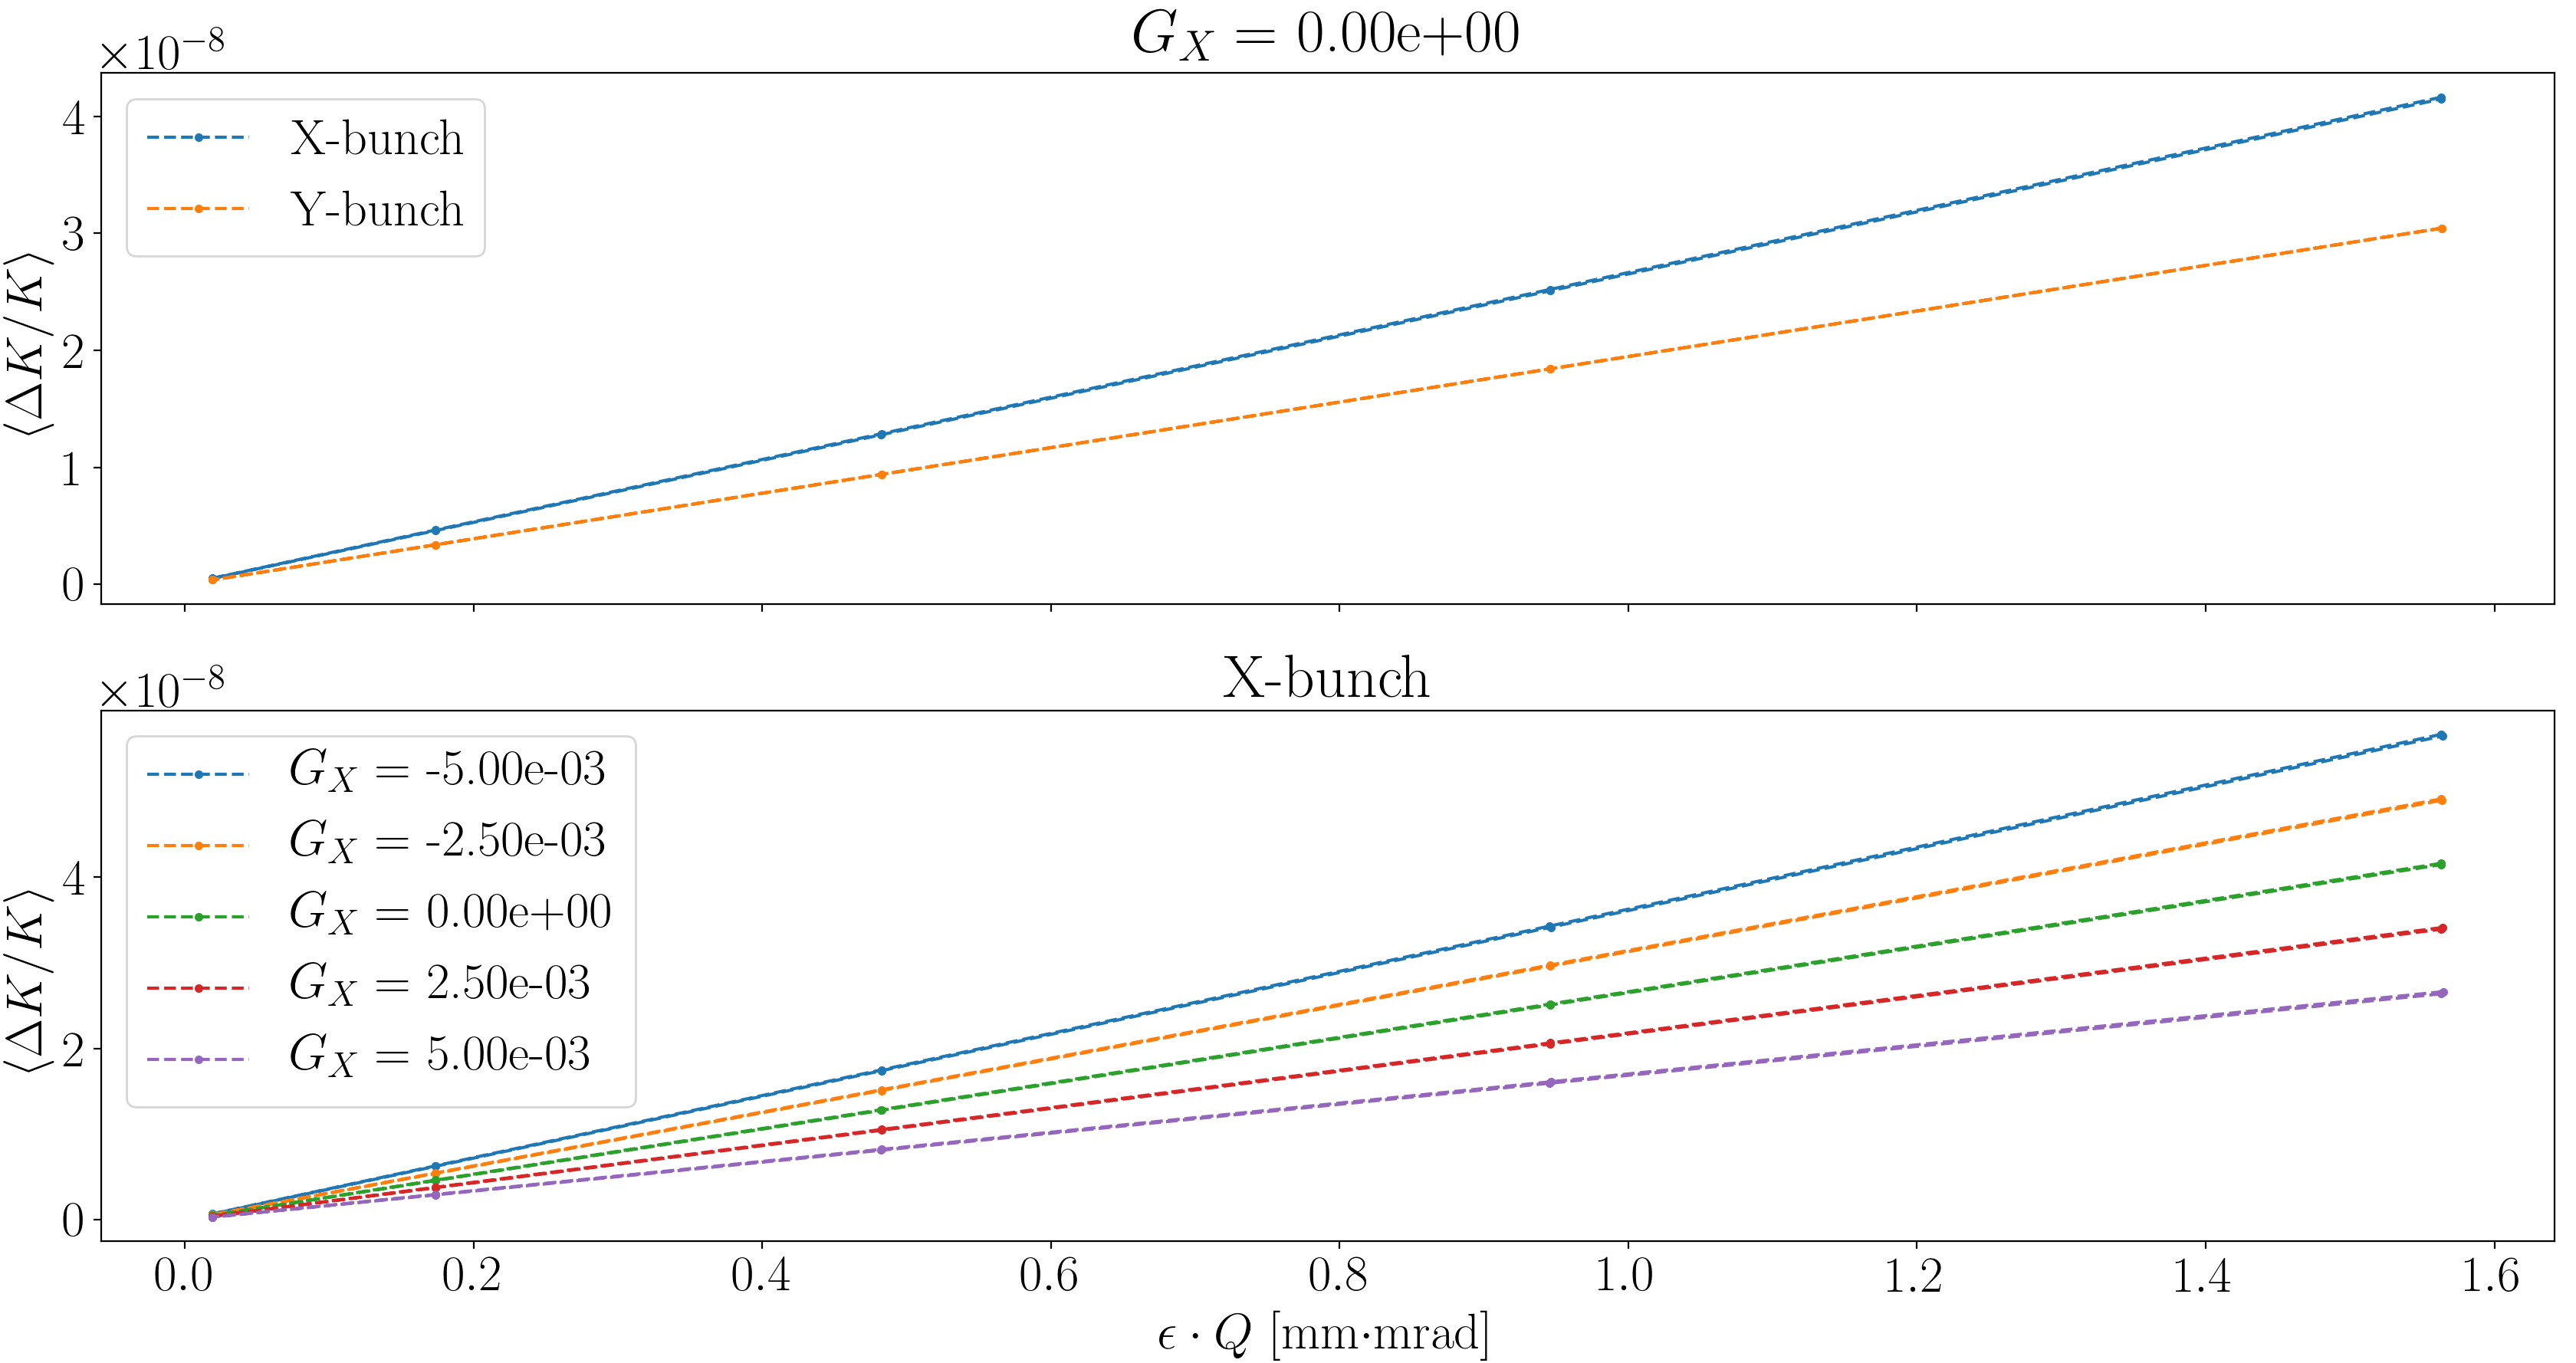
\includegraphics[height=.3\paperheight]{images/stune_traj_equ/part1/equ_energy_vs_emittance}
	\caption{Longitudinal emittance dependence of the mean energy level.\label{fig:equ_nrg_vs_emittance}}
\end{figure}

The observed longitudinal dependence of the momentum compaction factor is further confirmed by equation~(15)
of reference~\cite{Senichev:IPAC13}, in which we find:
\[
\alpha_0 = \avg{\frac{D_0}{\rho}},~~ \alpha_1 = \avg{\frac{D_1}{\rho}} + \frac12\avg{D_0'^2},
\]
where $D(s) = D_0(s) + D_1(s)\cdot \delta$  is the dispersion function, $\rho$ the radius of the clsed orbit.
In first approximation, dispersion exists only in the horizontal plane and is zero in the vertical plane,
meaning that the spatial dependence of the dispersion function reflects on the spatial dependence of the momentum
compaction factor.

For comparison, the same tests were carried out with linear Taylor expansions of the spin and orbital
transfer maps. The results are shown in Figures~\ref{fig:stune_traj_equ_linear:stune_vs_nrg},
and~\ref{fig:stune_traj_equ_linear:nrg_vs_emittance}. As one can see in
Figure~\ref{fig:stune_traj_equ_linear:nrg_vs_emittance}, all particles doing betatron oscillations in the
vertical plane share the same value of the mean energy level, which is an indication that they share
the same closed orbit, which in turn means there's no dispersion in the vertical plane.
In this case, from Figure~\ref{fig:stune_traj_equ_linear:stune_vs_nrg} follows that their spin tunes
are equal.

\begin{figure}[h]
\centering
\begin{subfigure}{\linewidth}
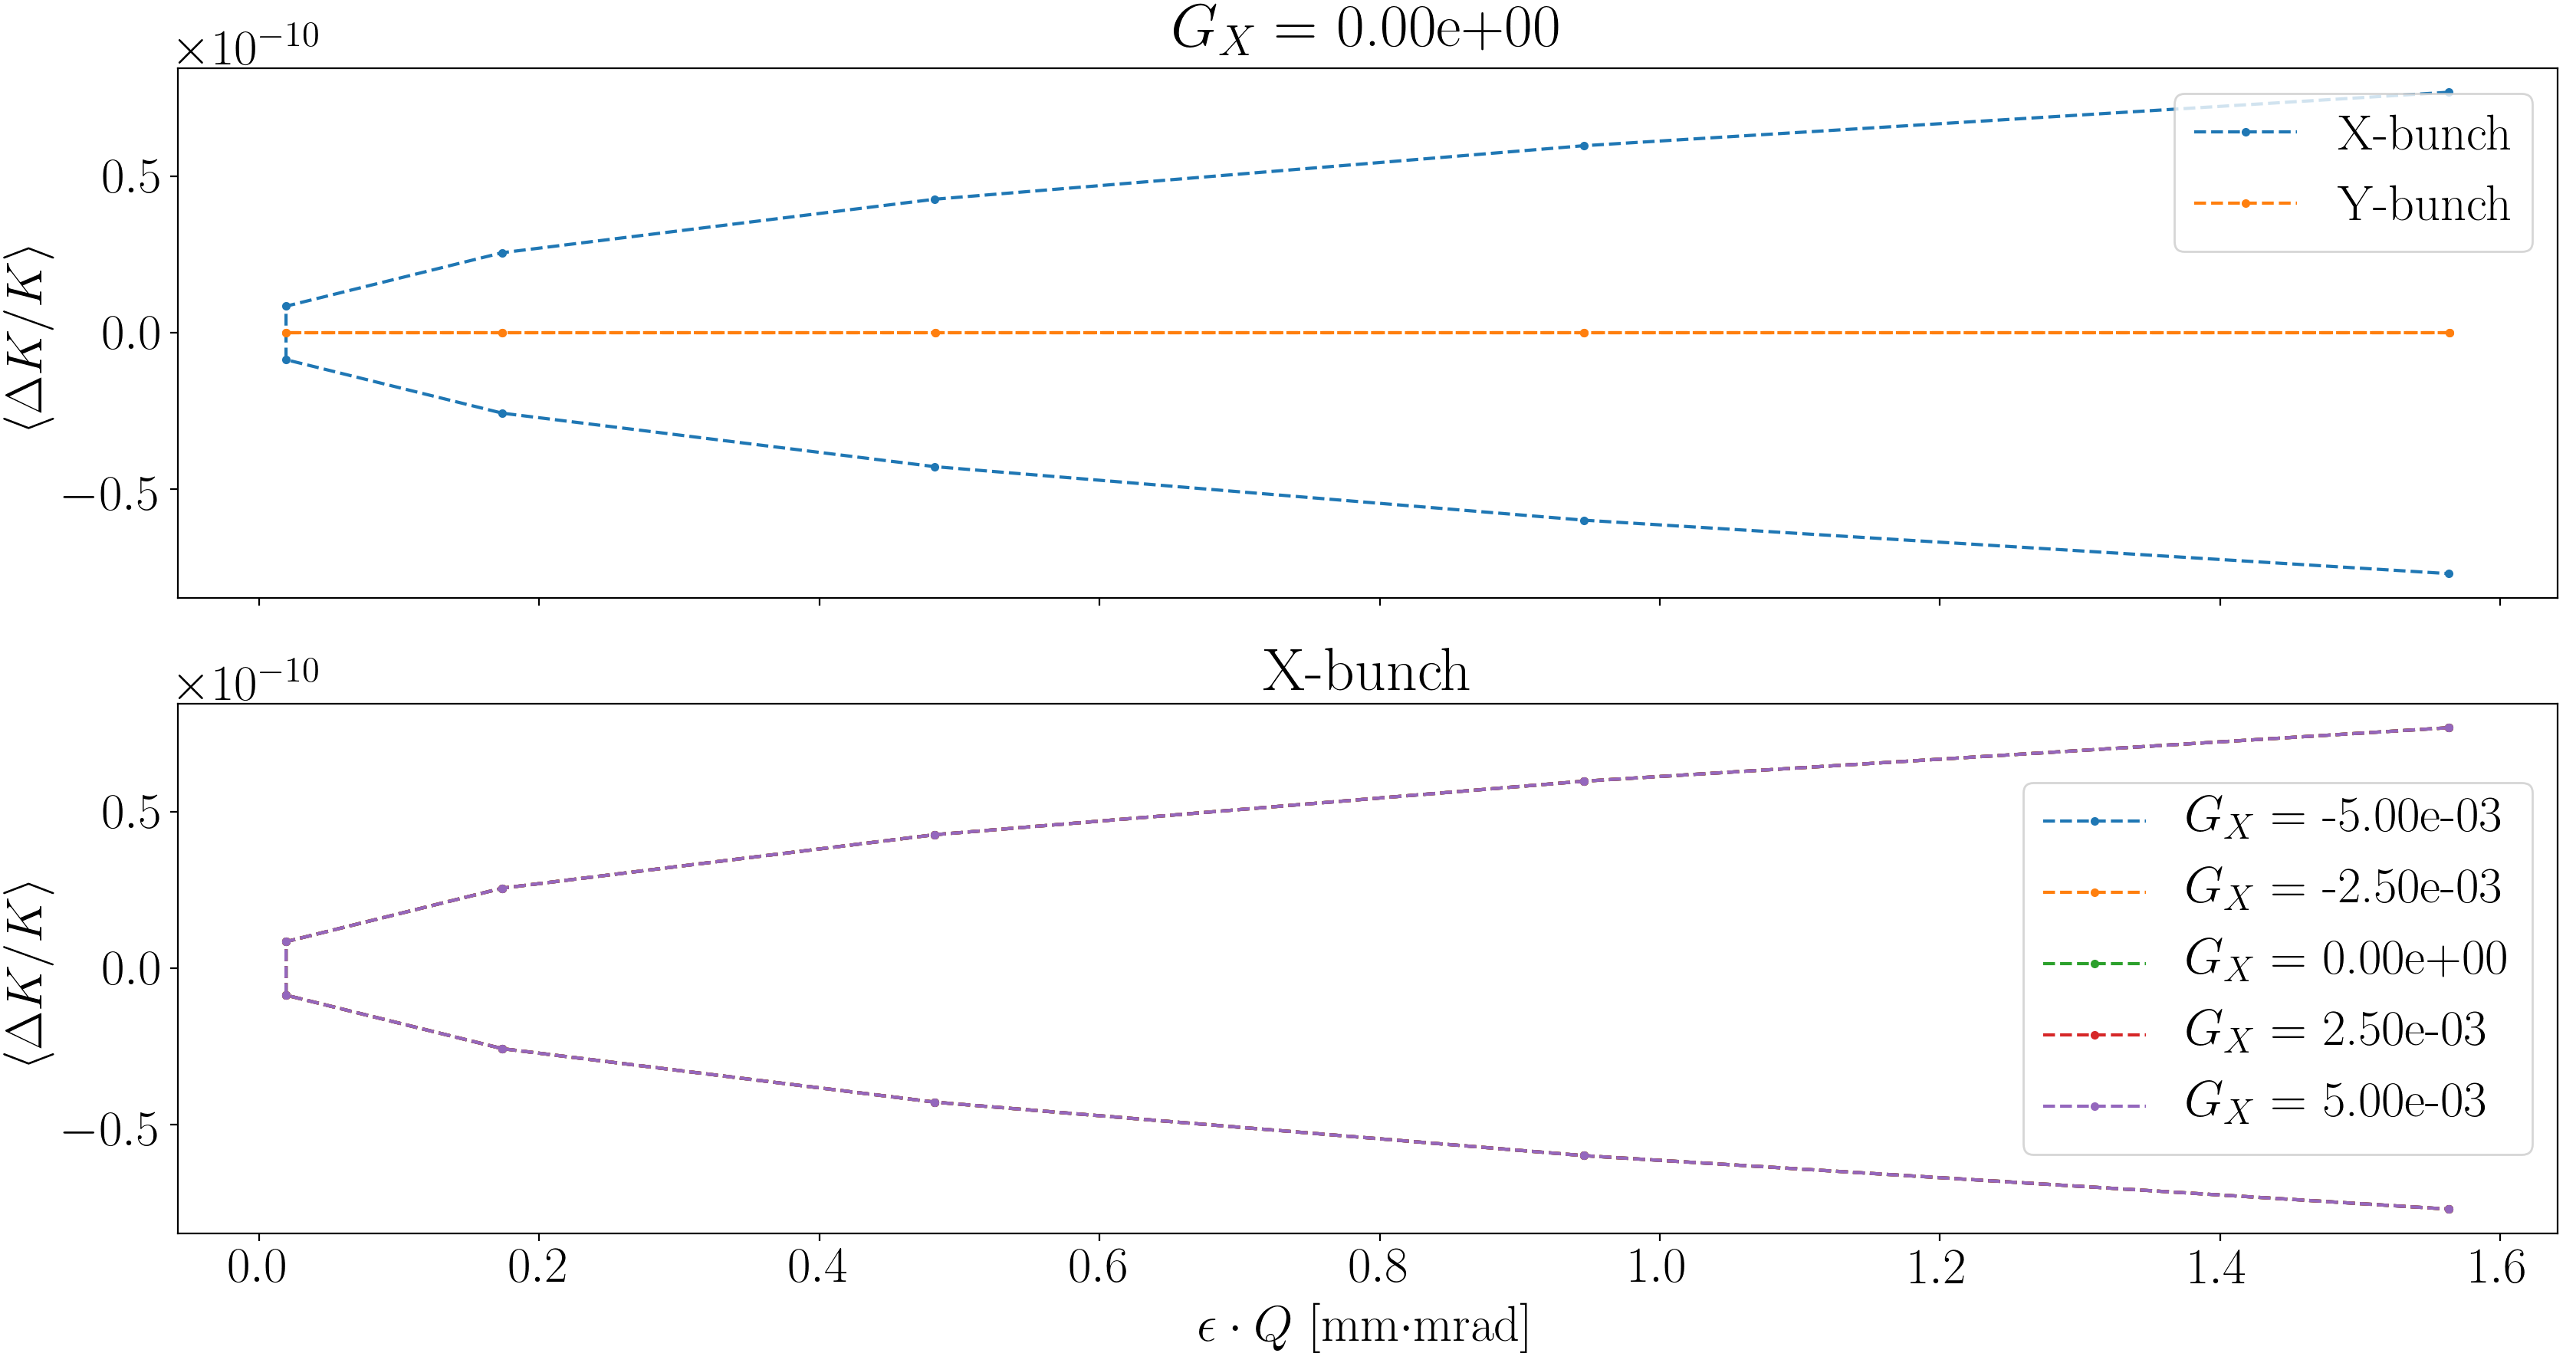
\includegraphics[width=\linewidth]{images/stune_traj_equ/part1/equ_energy_vs_emittance_linear}
\caption{Mean energy level dependence on
particle transverse emittance\label{fig:stune_traj_equ_linear:nrg_vs_emittance}}
\end{subfigure} 
\begin{subfigure}{\linewidth}
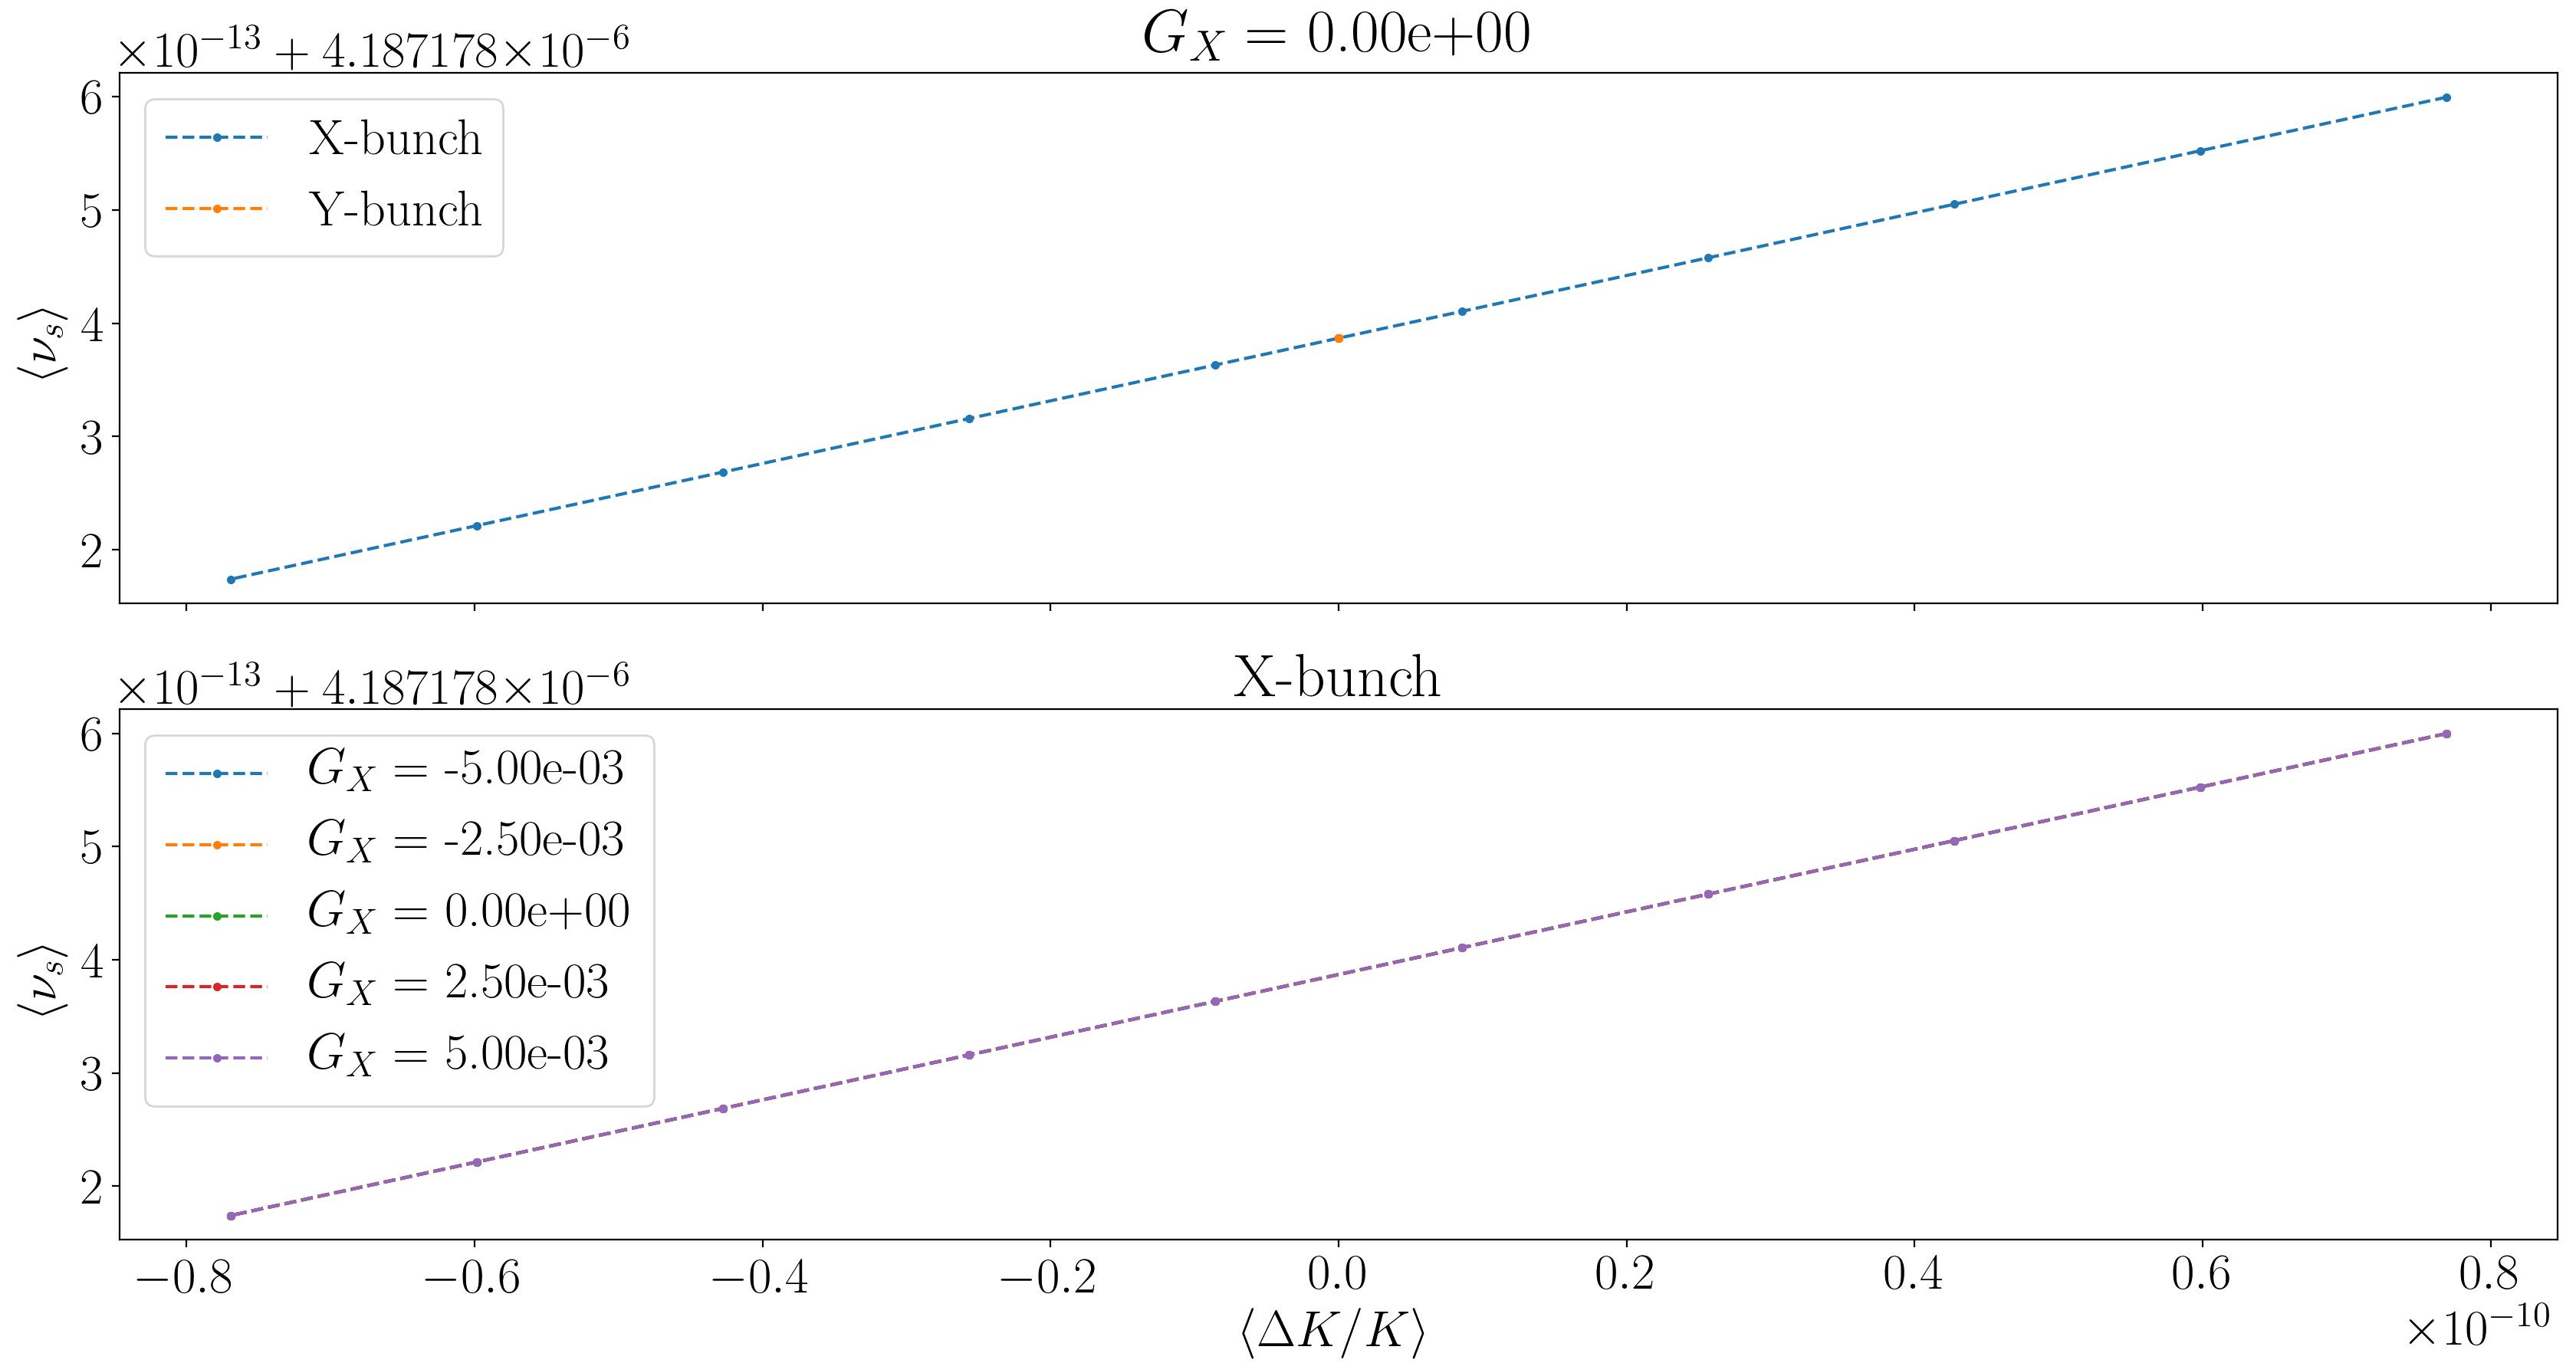
\includegraphics[width=\linewidth]{images/stune_traj_equ/part1/stune_vs_equ_energy_linear}
\caption{Mean spin tune dependence on mean energy.\label{fig:stune_traj_equ_linear:stune_vs_nrg}}
\end{subfigure} 
\caption{Simulation results in the case of linear transfer maps.}
\end{figure}

In Figure~\ref{fig:long_emitt_vs_trans_emitt} are plotted the particle longitudinal emittance as a
function of its Q-normalized transverse emittance. As one can see, the transverse emittances induce
the longitudianl emittances at different rates, depending on the betatron oscillation plane.
In the linear case, vertical plane betatron oscillations do not induce synchrotron oscillations at all.
\begin{figure}[h]
\centering
\begin{subfigure}{\linewidth}
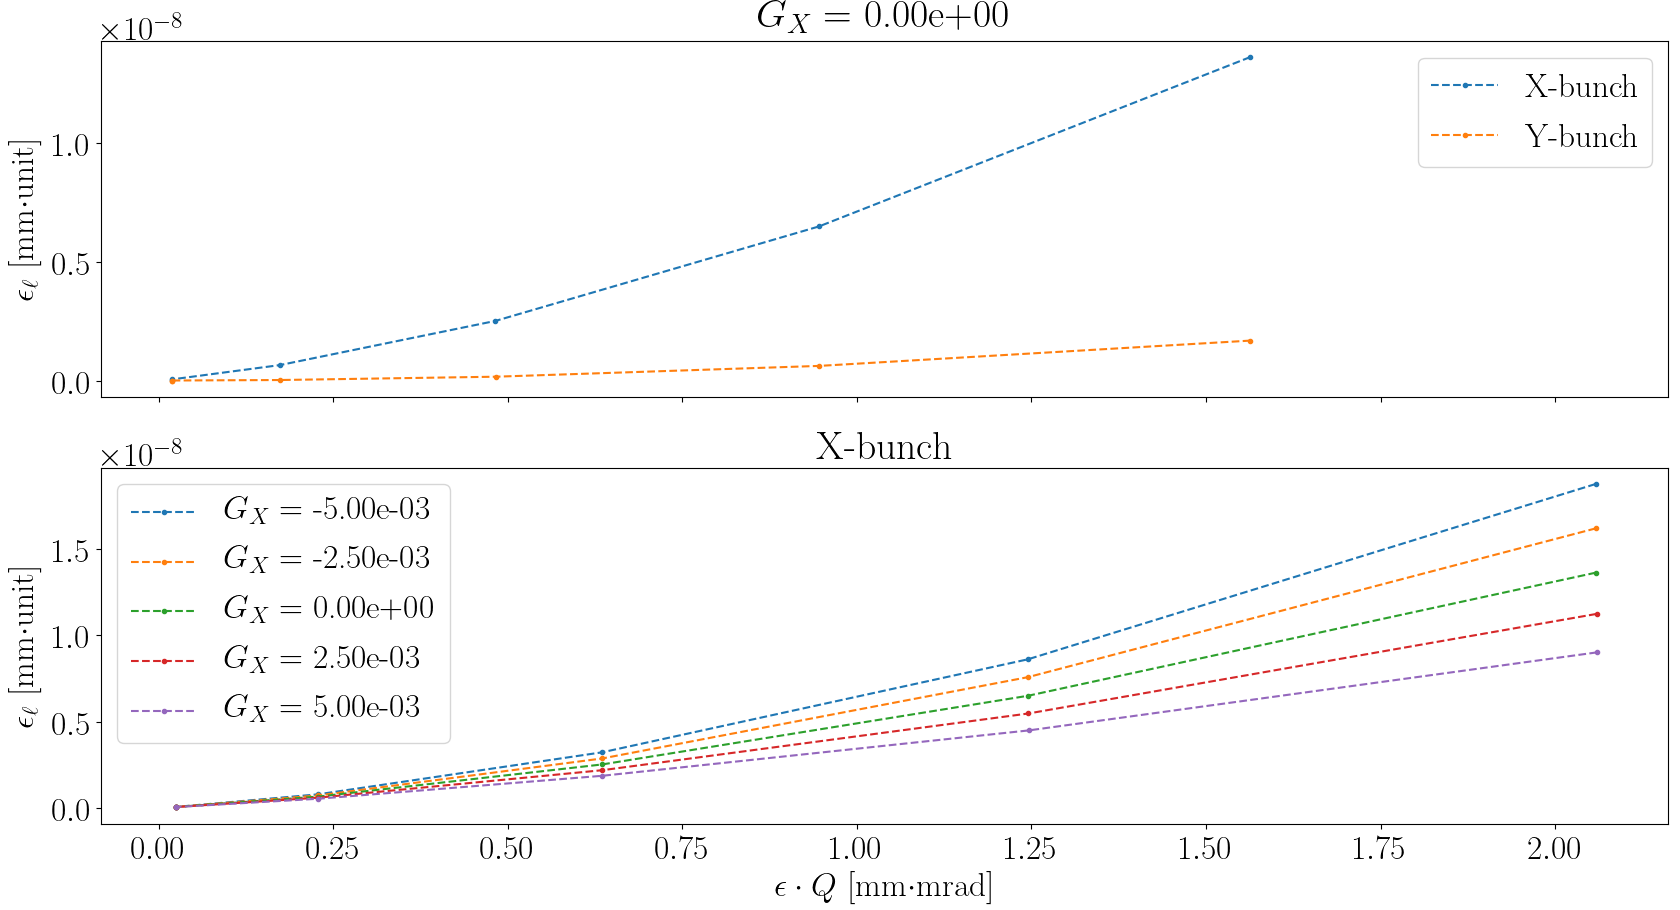
\includegraphics[height=.3\paperheight]{images/stune_traj_equ/part1/long_emitt_vs_trans_emitt}
\caption{Non-linear transfer maps.}
\end{subfigure}
\begin{subfigure}{\linewidth}
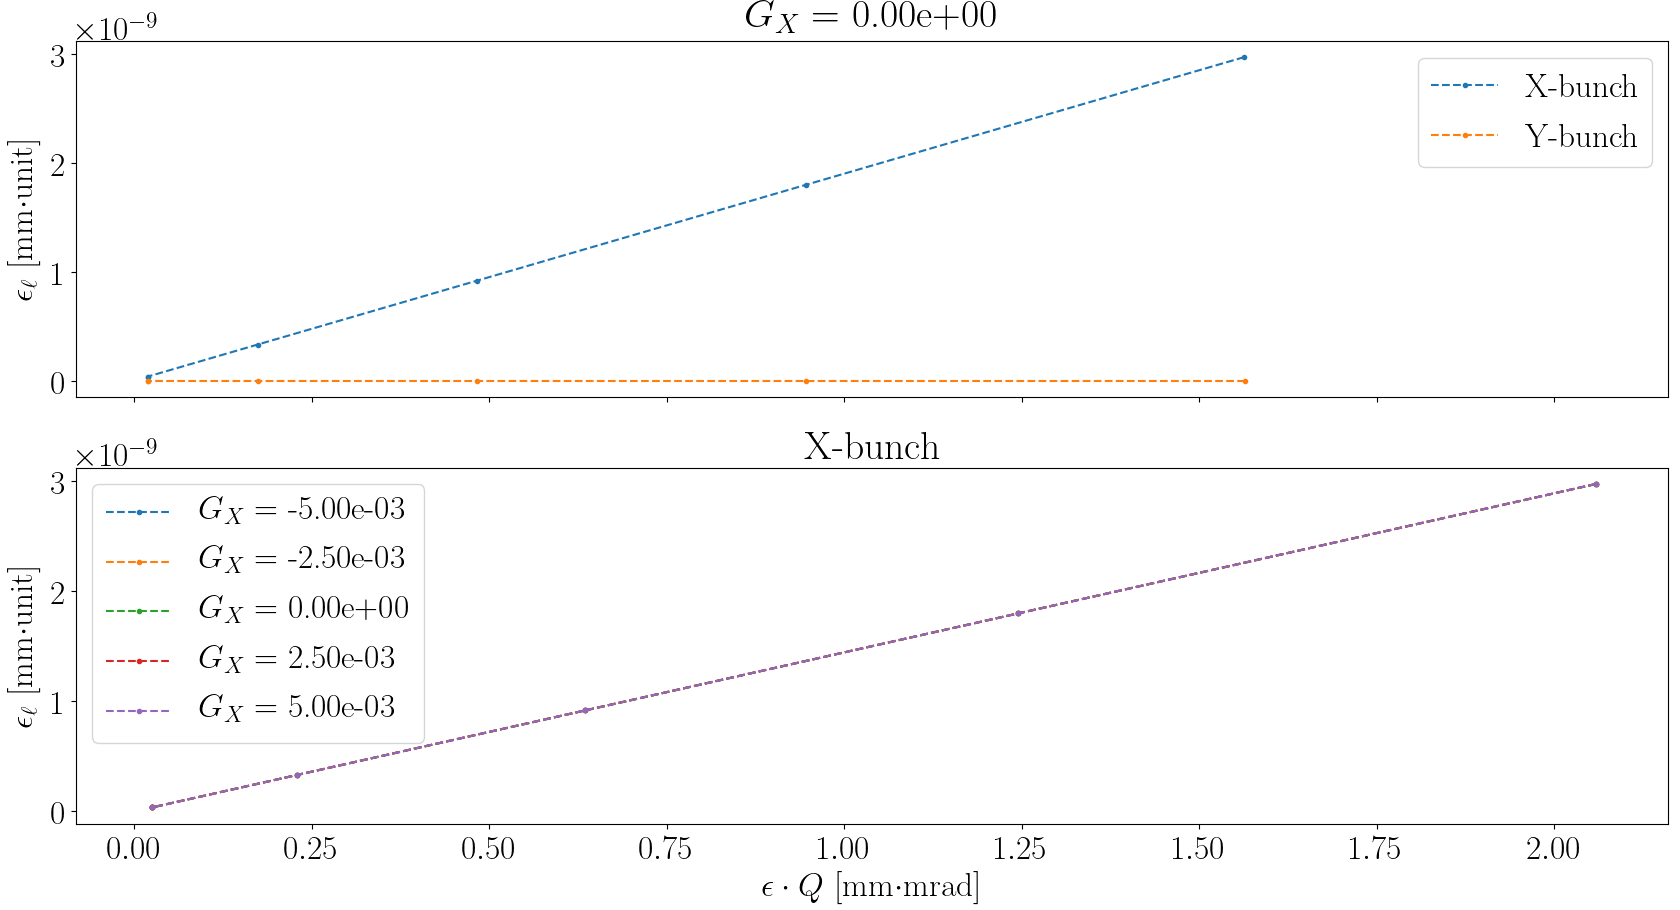
\includegraphics[height=.3\paperheight]{images/stune_traj_equ/part1/long_emitt_vs_trans_emitt_linear}
\caption{Linear transfer maps.}
\end{subfigure}
\caption{Longitudinal emittance as a function of
Q-normalized transverse emittance.\label{fig:long_emitt_vs_trans_emitt}}
\end{figure}

\paragraph{Conclusion:} formulation A of Statement 1 is false. 


\subsection{Formulation B}\label{sec:spin_stune_traj_equ:B_form}
\newcommand{\Ps}{\mathcal P}

Usinf COSY Infinity we compute the Taylor expantion of spin tune $\nu_s(\vec z)$, where
\begin{align*}
  \vec z &= (x,a,y,b,\ell,\delta), \\
  \ell &= -(t - t_0)v_0\frac{\gamma-1}{\gamma}, \\
  \delta &= \frac{\Delta K}{K}.
\end{align*}

In the present section we will test formulation B of Statement 1:
the multivariate function $\nu_s(\vec z)$ can be expressed as a function of a single scalar parameter
$\nu_s(\g*)$. We will not assume any formal expression of $\g*$.

If formulation B is correct, there exists a coordinate system (with one axis being $\nu_s$),
in which horizontal plane betatron oscillating particles are indistinguishable, in terms of spin tune,
from vertical plane betatron oscillating particles. This coordinate system, hence, must not include
coordinates from the transverse phase space planes $(x,a)$, and $(y,b)$.

Therefore, we will look at the space $\Ps=(\ell, \delta, \nu_s)$. If formulation B is correct,
differences between particles' transverse phase plane trajectories must not reflect on their
trajetctories in $\Ps$.

We used the same data in this analysis as in the previous section.

In Figure~\ref{fig:main:all_ps} $\nu_s(\vec z)$ is plotted as a function of $(\ell, \delta)$ when
$\vec z$ is the real trajectory the particle takes in the storage ring. We observe:
\begin{enumerate}
\item the same stratification of the mean spin tune levels as in section~\ref{sec:decoh:sim-imperfect};
  \item the stratification if more pronounced for the X-bunch (blue dots), than for the Y-bunch (red dots).
\end{enumerate}

The latter can be explained by thee greater magnitude of the dispersion function in the horizontal plane.
Note that at equal values of the Q-normalized transverse emittance~\footnote{Q-normalized is $\epsilon_\alpha\cdot Q_\alpha$, where $\alpha\in\{x,y\}$.} (i.e. at equal orbit lengthenings, if equation~\eqref{eq:betatron_OL}
is to be believed), horizontal plane betatron oscillating particles have a greater longitudinal emittance than
those oscillating in the vertical plane.

\begin{figure}[h]
  \centering
  \begin{subfigure}{\linewidth}
    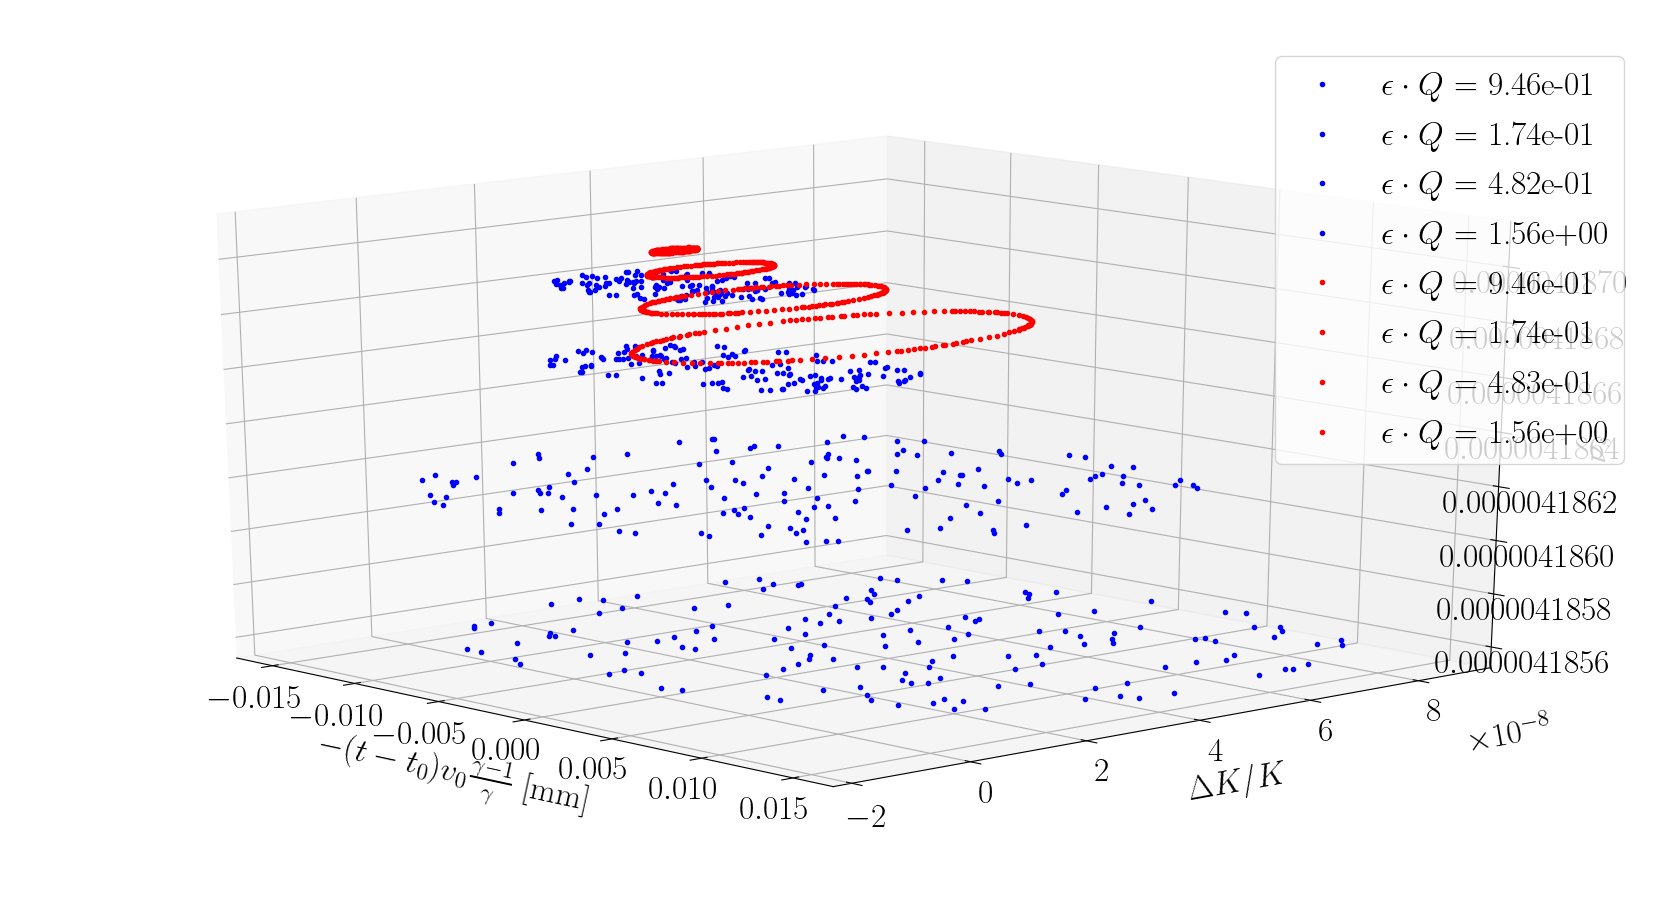
\includegraphics[height=.3\paperheight]{images/stune_traj_equ/part2/3D_plot_all_ps_vars}
    \caption{Particles picked according to the values of their Q-normalized \emph{transverse}
    emittances.\label{fig:main:all_ps}}
  \end{subfigure}
  \begin{subfigure}{\linewidth}
    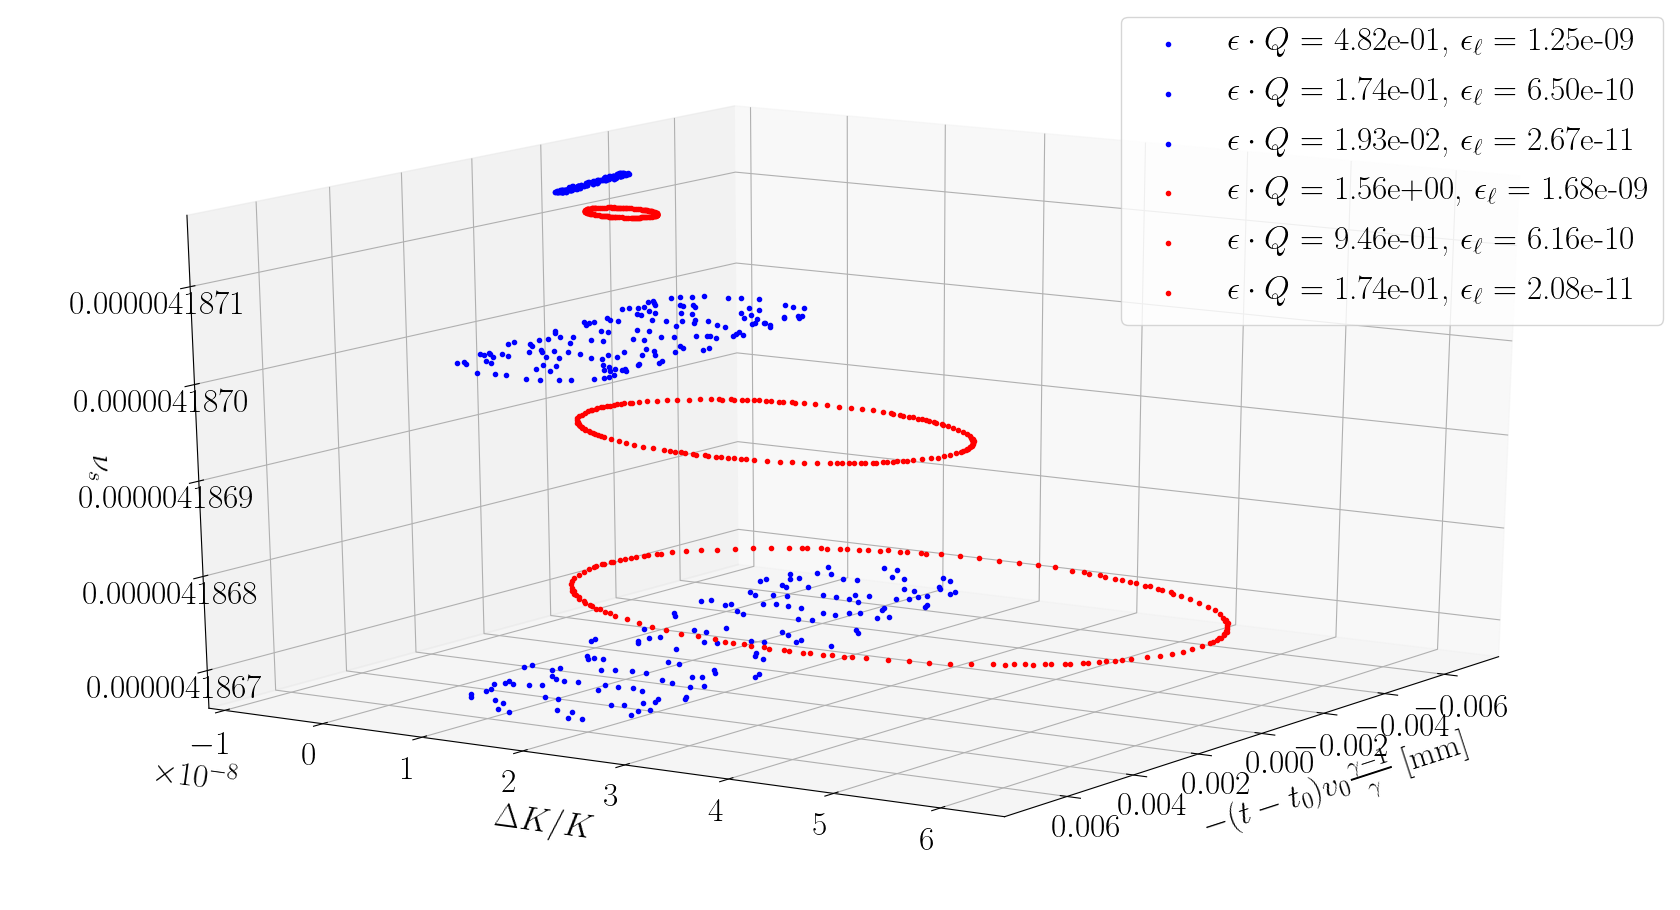
\includegraphics[height=.3\paperheight]{images/stune_traj_equ/part2/3D_plot_all_ps_vars_equal_long_emi}
    \caption{Particles are picked according to the values of their \emph{longitudinal}
    emittances.\label{fig:main:gamma_eff}}
  \end{subfigure}
  \caption{Spin tune as a function of the particle's position in the longitudinal phase space.
    Colors mark the bunch: blue for X, red for Y. The corresponding Q-normalized transverse and
    longitudinal emittances are shown in the legend.\label{fig:main}}
\end{figure}

Due to the latter fact, we decided to plot the same dependence, but to pick particles based on the equality of
their longitudinal, instead of transverse, emittances. In Figure~\ref{fig:main:gamma_eff} we observe that
particles having similar magnitudes of their longitudinal emittance have also silimar mean spin tune levels.

\paragraph{Conclusion:} formulation B is confirmed by simulation; the effective Lorentz factor reflects the
magnitude of the particle's longitudinal emittance.

In view of Figure~\ref{decoh:fig:nbar_vs_ST}, one can also conclude that particles with equal
effective L-factor values are spin dynamics-equivalent in the general sense, by which we mean that
they have not only equal values of spin tune, but the same orientation of the invariant spin axis.~\footnote{
At any rate, this seems to be true in the FS regime of operation.}


\clearpage
